\documentclass[twoside]{book}

% Packages required by doxygen
\usepackage{fixltx2e}
\usepackage{calc}
\usepackage{doxygen}
\usepackage[export]{adjustbox} % also loads graphicx
\usepackage{graphicx}
\usepackage[utf8]{inputenc}
\usepackage{makeidx}
\usepackage{multicol}
\usepackage{multirow}
\PassOptionsToPackage{warn}{textcomp}
\usepackage{textcomp}
\usepackage[nointegrals]{wasysym}
\usepackage[table]{xcolor}

% Font selection
\usepackage[T1]{fontenc}
\usepackage[scaled=.90]{helvet}
\usepackage{courier}
\usepackage{amssymb}
\usepackage{sectsty}
\renewcommand{\familydefault}{\sfdefault}
\allsectionsfont{%
  \fontseries{bc}\selectfont%
  \color{darkgray}%
}
\renewcommand{\DoxyLabelFont}{%
  \fontseries{bc}\selectfont%
  \color{darkgray}%
}
\newcommand{\+}{\discretionary{\mbox{\scriptsize$\hookleftarrow$}}{}{}}

% Page & text layout
\usepackage{geometry}
\geometry{%
  a4paper,%
  top=2.5cm,%
  bottom=2.5cm,%
  left=2.5cm,%
  right=2.5cm%
}
\tolerance=750
\hfuzz=15pt
\hbadness=750
\setlength{\emergencystretch}{15pt}
\setlength{\parindent}{0cm}
\setlength{\parskip}{3ex plus 2ex minus 2ex}
\makeatletter
\renewcommand{\paragraph}{%
  \@startsection{paragraph}{4}{0ex}{-1.0ex}{1.0ex}{%
    \normalfont\normalsize\bfseries\SS@parafont%
  }%
}
\renewcommand{\subparagraph}{%
  \@startsection{subparagraph}{5}{0ex}{-1.0ex}{1.0ex}{%
    \normalfont\normalsize\bfseries\SS@subparafont%
  }%
}
\makeatother

% Headers & footers
\usepackage{fancyhdr}
\pagestyle{fancyplain}
\fancyhead[LE]{\fancyplain{}{\bfseries\thepage}}
\fancyhead[CE]{\fancyplain{}{}}
\fancyhead[RE]{\fancyplain{}{\bfseries\leftmark}}
\fancyhead[LO]{\fancyplain{}{\bfseries\rightmark}}
\fancyhead[CO]{\fancyplain{}{}}
\fancyhead[RO]{\fancyplain{}{\bfseries\thepage}}
\fancyfoot[LE]{\fancyplain{}{}}
\fancyfoot[CE]{\fancyplain{}{}}
\fancyfoot[RE]{\fancyplain{}{\bfseries\scriptsize Generated by Doxygen }}
\fancyfoot[LO]{\fancyplain{}{\bfseries\scriptsize Generated by Doxygen }}
\fancyfoot[CO]{\fancyplain{}{}}
\fancyfoot[RO]{\fancyplain{}{}}
\renewcommand{\footrulewidth}{0.4pt}
\renewcommand{\chaptermark}[1]{%
  \markboth{#1}{}%
}
\renewcommand{\sectionmark}[1]{%
  \markright{\thesection\ #1}%
}

% Indices & bibliography
\usepackage{natbib}
\usepackage[titles]{tocloft}
\setcounter{tocdepth}{3}
\setcounter{secnumdepth}{5}
\makeindex

% Hyperlinks (required, but should be loaded last)
\usepackage{ifpdf}
\ifpdf
  \usepackage[pdftex,pagebackref=true]{hyperref}
\else
  \usepackage[ps2pdf,pagebackref=true]{hyperref}
\fi
\hypersetup{%
  colorlinks=true,%
  linkcolor=blue,%
  citecolor=blue,%
  unicode%
}

% Custom commands
\newcommand{\clearemptydoublepage}{%
  \newpage{\pagestyle{empty}\cleardoublepage}%
}

\usepackage{caption}
\captionsetup{labelsep=space,justification=centering,font={bf},singlelinecheck=off,skip=4pt,position=top}

%===== C O N T E N T S =====

\begin{document}

% Titlepage & ToC
\hypersetup{pageanchor=false,
             bookmarksnumbered=true,
             pdfencoding=unicode
            }
\pagenumbering{alph}
\begin{titlepage}
\vspace*{7cm}
\begin{center}%
{\Large Ten\+Ten \\[1ex]\large 2.\+1.\+0 }\\
\vspace*{1cm}
{\large Generated by Doxygen 1.8.12}\\
\end{center}
\end{titlepage}
\clearemptydoublepage
\pagenumbering{roman}
\tableofcontents
\clearemptydoublepage
\pagenumbering{arabic}
\hypersetup{pageanchor=true}

%--- Begin generated contents ---
\chapter{Hierarchical Index}
\section{Class Hierarchy}
This inheritance list is sorted roughly, but not completely, alphabetically\+:\begin{DoxyCompactList}
\item \contentsline{section}{Board}{\pageref{class_board}}{}
\item exception\begin{DoxyCompactList}
\item \contentsline{section}{syntax\+\_\+exception}{\pageref{classsyntax__exception}}{}
\end{DoxyCompactList}
\item \contentsline{section}{Form}{\pageref{class_form}}{}
\item \contentsline{section}{global\+Log}{\pageref{classglobal_log}}{}
\item \contentsline{section}{main\+Game}{\pageref{classmain_game}}{}
\item \contentsline{section}{Option}{\pageref{class_option}}{}
\item \contentsline{section}{Option\+Set}{\pageref{class_option_set}}{}
\item \contentsline{section}{Point}{\pageref{struct_point}}{}
\end{DoxyCompactList}

\chapter{Class Index}
\section{Class List}
Here are the classes, structs, unions and interfaces with brief descriptions\+:\begin{DoxyCompactList}
\item\contentsline{section}{\hyperlink{class_board}{Board} \\*\hyperlink{class_board}{Board} class }{\pageref{class_board}}{}
\item\contentsline{section}{\hyperlink{class_form}{Form} \\*\hyperlink{class_form}{Form} class }{\pageref{class_form}}{}
\item\contentsline{section}{\hyperlink{classglobal_log}{global\+Log} \\*Log class }{\pageref{classglobal_log}}{}
\item\contentsline{section}{\hyperlink{classmain_game}{main\+Game} \\*Main game class }{\pageref{classmain_game}}{}
\item\contentsline{section}{\hyperlink{class_option}{Option} \\*\hyperlink{class_option}{Option} class }{\pageref{class_option}}{}
\item\contentsline{section}{\hyperlink{class_option_set}{Option\+Set} \\*\hyperlink{class_option}{Option} set class }{\pageref{class_option_set}}{}
\item\contentsline{section}{\hyperlink{struct_point}{Point} \\*\hyperlink{struct_point}{Point} structure }{\pageref{struct_point}}{}
\item\contentsline{section}{\hyperlink{classsyntax__exception}{syntax\+\_\+exception} \\*Config class }{\pageref{classsyntax__exception}}{}
\end{DoxyCompactList}

\chapter{File Index}
\section{File List}
Here is a list of all files with brief descriptions\+:\begin{DoxyCompactList}
\item\contentsline{section}{\hyperlink{board_8cpp}{board.\+cpp} }{\pageref{board_8cpp}}{}
\item\contentsline{section}{\hyperlink{board_8h}{board.\+h} }{\pageref{board_8h}}{}
\item\contentsline{section}{\hyperlink{color_8cpp}{color.\+cpp} }{\pageref{color_8cpp}}{}
\item\contentsline{section}{\hyperlink{color_8h}{color.\+h} }{\pageref{color_8h}}{}
\item\contentsline{section}{\hyperlink{config__load_8cpp}{config\+\_\+load.\+cpp} }{\pageref{config__load_8cpp}}{}
\item\contentsline{section}{\hyperlink{config__load_8h}{config\+\_\+load.\+h} }{\pageref{config__load_8h}}{}
\item\contentsline{section}{\hyperlink{form_8cpp}{form.\+cpp} }{\pageref{form_8cpp}}{}
\item\contentsline{section}{\hyperlink{form_8h}{form.\+h} }{\pageref{form_8h}}{}
\item\contentsline{section}{\hyperlink{game__window_8cpp}{game\+\_\+window.\+cpp} }{\pageref{game__window_8cpp}}{}
\item\contentsline{section}{\hyperlink{game__window_8h}{game\+\_\+window.\+h} }{\pageref{game__window_8h}}{}
\item\contentsline{section}{\hyperlink{global__log_8cpp}{global\+\_\+log.\+cpp} }{\pageref{global__log_8cpp}}{}
\item\contentsline{section}{\hyperlink{global__log_8h}{global\+\_\+log.\+h} }{\pageref{global__log_8h}}{}
\item\contentsline{section}{\hyperlink{include_g_u_i_8h}{include\+G\+U\+I.\+h} }{\pageref{include_g_u_i_8h}}{}
\item\contentsline{section}{\hyperlink{main_8cpp}{main.\+cpp} }{\pageref{main_8cpp}}{}
\item\contentsline{section}{\hyperlink{main__game_8cpp}{main\+\_\+game.\+cpp} }{\pageref{main__game_8cpp}}{}
\item\contentsline{section}{\hyperlink{main__game_8h}{main\+\_\+game.\+h} }{\pageref{main__game_8h}}{}
\item\contentsline{section}{\hyperlink{main__window_8cpp}{main\+\_\+window.\+cpp} }{\pageref{main__window_8cpp}}{}
\item\contentsline{section}{\hyperlink{main__window_8h}{main\+\_\+window.\+h} }{\pageref{main__window_8h}}{}
\item\contentsline{section}{\hyperlink{menu__window_8cpp}{menu\+\_\+window.\+cpp} }{\pageref{menu__window_8cpp}}{}
\item\contentsline{section}{\hyperlink{menu__window_8h}{menu\+\_\+window.\+h} }{\pageref{menu__window_8h}}{}
\item\contentsline{section}{\hyperlink{option_8cpp}{option.\+cpp} }{\pageref{option_8cpp}}{}
\item\contentsline{section}{\hyperlink{option_8h}{option.\+h} }{\pageref{option_8h}}{}
\end{DoxyCompactList}

\chapter{Class Documentation}
\hypertarget{class_board}{}\section{Board Class Reference}
\label{class_board}\index{Board@{Board}}


\hyperlink{class_board}{Board} class.  




{\ttfamily \#include $<$board.\+h$>$}

\subsection*{Public Member Functions}
\begin{DoxyCompactItemize}
\item 
\hyperlink{class_board_a815539526352256b76c07aaeb633dbb7}{Board} (int \+\_\+width, int \+\_\+height)
\begin{DoxyCompactList}\small\item\em Constructor. \end{DoxyCompactList}\item 
\hyperlink{class_board_a467d2914714aa66a5b29e963ea4bf30b}{Board} (const \hyperlink{class_board}{Board} \&\+\_\+board)
\begin{DoxyCompactList}\small\item\em Constructor by copy. \end{DoxyCompactList}\item 
\hyperlink{class_board_af73f45730119a1fd8f6670f53f959e68}{$\sim$\+Board} ()
\begin{DoxyCompactList}\small\item\em Destructor. \end{DoxyCompactList}\item 
\hyperlink{class_board}{Board} \& \hyperlink{class_board_ac67493bc18a85bffd6d31b294e0298b9}{operator=} (const \hyperlink{class_board}{Board} \&\+\_\+board)
\begin{DoxyCompactList}\small\item\em Overload of affectation operator. \end{DoxyCompactList}\item 
void \hyperlink{class_board_a0380aba58e451b88ec206e253083e049}{set\+Square} (int x, int y, int color)
\begin{DoxyCompactList}\small\item\em Change a square\textquotesingle{}s color. \end{DoxyCompactList}\item 
void \hyperlink{class_board_a533f62eccb7919cd20aba0ae9ea0e790}{add\+Form} (const \hyperlink{class_form}{Form} \&form, int x, int y, int color)
\begin{DoxyCompactList}\small\item\em Put a shape on the board. \end{DoxyCompactList}\item 
bool \hyperlink{class_board_a6daa08c6ef14e1935538a749a6062913}{form\+Collide} (const \hyperlink{class_form}{Form} \&form, int x, int y) const
\begin{DoxyCompactList}\small\item\em Check if a form can be place on the board. \end{DoxyCompactList}\item 
void \hyperlink{class_board_ad4c85c20b50431a292293f38f412436a}{clean} (int \&\+\_\+line, int \&\+\_\+column)
\begin{DoxyCompactList}\small\item\em Clean filled lignes and columns. \end{DoxyCompactList}\item 
const int $\ast$ \hyperlink{class_board_a92d07d150ac4f9c341fd18168d86072c}{operator\mbox{[}$\,$\mbox{]}} (int n) const
\begin{DoxyCompactList}\small\item\em Access operator. \end{DoxyCompactList}\item 
int \hyperlink{class_board_a503f6433c6b70b70d79a775f53a46d77}{getwidth} () const
\begin{DoxyCompactList}\small\item\em Accessor in reading of the width. \end{DoxyCompactList}\item 
int \hyperlink{class_board_aafa14471fcdcd50b0edb336d4454b40c}{getheight} () const
\begin{DoxyCompactList}\small\item\em Accessor in reading of the height. \end{DoxyCompactList}\item 
std\+::string \hyperlink{class_board_a57166342ac5109301eba30a452c515af}{write} () const
\begin{DoxyCompactList}\small\item\em Write board. \end{DoxyCompactList}\item 
void \hyperlink{class_board_a32cb3d0839fd2abceb1ffcba270ae4fd}{read} (const std\+::string \&str)
\begin{DoxyCompactList}\small\item\em Read a configuration form a string. \end{DoxyCompactList}\end{DoxyCompactItemize}


\subsection{Detailed Description}
\hyperlink{class_board}{Board} class. 

This class defines the main 1010 board. It mostly is the array of squares with all method required to manipulate it 

Definition at line 27 of file board.\+h.



\subsection{Constructor \& Destructor Documentation}
\hypertarget{class_board_a815539526352256b76c07aaeb633dbb7}{}\label{class_board_a815539526352256b76c07aaeb633dbb7} 
\index{Board@{Board}!Board@{Board}}
\index{Board@{Board}!Board@{Board}}
\subsubsection{\texorpdfstring{Board()}{Board()}\hspace{0.1cm}{\footnotesize\ttfamily [1/2]}}
{\footnotesize\ttfamily Board\+::\+Board (\begin{DoxyParamCaption}\item[{int}]{\+\_\+width,  }\item[{int}]{\+\_\+height }\end{DoxyParamCaption})}



Constructor. 

Constructor for \hyperlink{class_board}{Board}

Set size then create array and initialize it empty.


\begin{DoxyParams}{Parameters}
{\em \+\_\+width} & \+: \hyperlink{class_board}{Board}\textquotesingle{}s width (number of possinble squares) \\
\hline
{\em \+\_\+height} & \+: \hyperlink{class_board}{Board}\textquotesingle{}s height (number of possible squares) \\
\hline
\end{DoxyParams}


Definition at line 6 of file board.\+cpp.

\hypertarget{class_board_a467d2914714aa66a5b29e963ea4bf30b}{}\label{class_board_a467d2914714aa66a5b29e963ea4bf30b} 
\index{Board@{Board}!Board@{Board}}
\index{Board@{Board}!Board@{Board}}
\subsubsection{\texorpdfstring{Board()}{Board()}\hspace{0.1cm}{\footnotesize\ttfamily [2/2]}}
{\footnotesize\ttfamily Board\+::\+Board (\begin{DoxyParamCaption}\item[{const \hyperlink{class_board}{Board} \&}]{\+\_\+board }\end{DoxyParamCaption})}



Constructor by copy. 

Constructor by copy of Baord class. Allow to build a board from another already existing. Set size then create the array witch is initialized with copied array\textquotesingle{}s values.


\begin{DoxyParams}{Parameters}
{\em \+\_\+board} & \+: \hyperlink{class_board}{Board} to copy \\
\hline
\end{DoxyParams}


Definition at line 19 of file board.\+cpp.

\hypertarget{class_board_af73f45730119a1fd8f6670f53f959e68}{}\label{class_board_af73f45730119a1fd8f6670f53f959e68} 
\index{Board@{Board}!````~Board@{$\sim$\+Board}}
\index{````~Board@{$\sim$\+Board}!Board@{Board}}
\subsubsection{\texorpdfstring{$\sim$\+Board()}{~Board()}}
{\footnotesize\ttfamily Board\+::$\sim$\+Board (\begin{DoxyParamCaption}{ }\end{DoxyParamCaption})}



Destructor. 

Baord of \hyperlink{class_board}{Board} instance (needed by presence of the dynamic allocation -\/2 dim. array-\/ in attribute). Free memory ligne by ligne then free main column. 

Definition at line 32 of file board.\+cpp.



\subsection{Member Function Documentation}
\hypertarget{class_board_a533f62eccb7919cd20aba0ae9ea0e790}{}\label{class_board_a533f62eccb7919cd20aba0ae9ea0e790} 
\index{Board@{Board}!add\+Form@{add\+Form}}
\index{add\+Form@{add\+Form}!Board@{Board}}
\subsubsection{\texorpdfstring{add\+Form()}{addForm()}}
{\footnotesize\ttfamily void Board\+::add\+Form (\begin{DoxyParamCaption}\item[{const \hyperlink{class_form}{Form} \&}]{form,  }\item[{int}]{x,  }\item[{int}]{y,  }\item[{int}]{color }\end{DoxyParamCaption})}



Put a shape on the board. 

Browse all squares used by the new form the add thoses squares one by one to the board.


\begin{DoxyParams}{Parameters}
{\em form} & \+: New form to add \\
\hline
{\em x} & \+: Abscissia where place the new form \\
\hline
{\em y} & \+: Ordinate where place the new form \\
\hline
{\em color} & \+: Color wished for this form \\
\hline
\end{DoxyParams}


Definition at line 69 of file board.\+cpp.

\hypertarget{class_board_ad4c85c20b50431a292293f38f412436a}{}\label{class_board_ad4c85c20b50431a292293f38f412436a} 
\index{Board@{Board}!clean@{clean}}
\index{clean@{clean}!Board@{Board}}
\subsubsection{\texorpdfstring{clean()}{clean()}}
{\footnotesize\ttfamily void Board\+::clean (\begin{DoxyParamCaption}\item[{int \&}]{\+\_\+line,  }\item[{int \&}]{\+\_\+column }\end{DoxyParamCaption})}



Clean filled lignes and columns. 

Browe every lign and column and mark whoses are filled. When it\textquotesingle{}s done, delete every marked line.


\begin{DoxyParams}{Parameters}
{\em \+\_\+ligne} & \+: Number of deleted lines \\
\hline
{\em \+\_\+column} & \+: Number of deleted columns \\
\hline
\end{DoxyParams}


Definition at line 99 of file board.\+cpp.

\hypertarget{class_board_a6daa08c6ef14e1935538a749a6062913}{}\label{class_board_a6daa08c6ef14e1935538a749a6062913} 
\index{Board@{Board}!form\+Collide@{form\+Collide}}
\index{form\+Collide@{form\+Collide}!Board@{Board}}
\subsubsection{\texorpdfstring{form\+Collide()}{formCollide()}}
{\footnotesize\ttfamily bool Board\+::form\+Collide (\begin{DoxyParamCaption}\item[{const \hyperlink{class_form}{Form} \&}]{form,  }\item[{int}]{x,  }\item[{int}]{y }\end{DoxyParamCaption}) const}



Check if a form can be place on the board. 

Get bounding box of the shape and check if it can be placed at coordinates passed as parameter. If the answer is yes then it need a more precise checking so it check squres one by one.


\begin{DoxyParams}{Parameters}
{\em form} & \+: Shape to verifie \\
\hline
{\em x} & \+: Abscissia where check collision \\
\hline
{\em y} & \+: Ordinate where check collision\\
\hline
\end{DoxyParams}
\begin{DoxyReturn}{Returns}
True if the shape can be place. 
\end{DoxyReturn}


Definition at line 80 of file board.\+cpp.

\hypertarget{class_board_aafa14471fcdcd50b0edb336d4454b40c}{}\label{class_board_aafa14471fcdcd50b0edb336d4454b40c} 
\index{Board@{Board}!getheight@{getheight}}
\index{getheight@{getheight}!Board@{Board}}
\subsubsection{\texorpdfstring{getheight()}{getheight()}}
{\footnotesize\ttfamily int Board\+::getheight (\begin{DoxyParamCaption}{ }\end{DoxyParamCaption}) const}



Accessor in reading of the height. 

\begin{DoxyReturn}{Returns}
The board\textquotesingle{}s heigtht 
\end{DoxyReturn}


Definition at line 163 of file board.\+cpp.

\hypertarget{class_board_a503f6433c6b70b70d79a775f53a46d77}{}\label{class_board_a503f6433c6b70b70d79a775f53a46d77} 
\index{Board@{Board}!getwidth@{getwidth}}
\index{getwidth@{getwidth}!Board@{Board}}
\subsubsection{\texorpdfstring{getwidth()}{getwidth()}}
{\footnotesize\ttfamily int Board\+::getwidth (\begin{DoxyParamCaption}{ }\end{DoxyParamCaption}) const}



Accessor in reading of the width. 

\begin{DoxyReturn}{Returns}
The board\textquotesingle{}s width 
\end{DoxyReturn}


Definition at line 159 of file board.\+cpp.

\hypertarget{class_board_ac67493bc18a85bffd6d31b294e0298b9}{}\label{class_board_ac67493bc18a85bffd6d31b294e0298b9} 
\index{Board@{Board}!operator=@{operator=}}
\index{operator=@{operator=}!Board@{Board}}
\subsubsection{\texorpdfstring{operator=()}{operator=()}}
{\footnotesize\ttfamily \hyperlink{class_board}{Board} \& Board\+::operator= (\begin{DoxyParamCaption}\item[{const \hyperlink{class_board}{Board} \&}]{\+\_\+board }\end{DoxyParamCaption})}



Overload of affectation operator. 

Affectation operator for \hyperlink{class_board}{Board} Allow to fully change the board from another board. Free memory ligne by ligne then free main column. Set size then create the array witch is initialized with copied array\textquotesingle{}s values.


\begin{DoxyParams}{Parameters}
{\em \+\_\+board} & \hyperlink{class_board}{Board} to be copied\\
\hline
\end{DoxyParams}
\begin{DoxyReturn}{Returns}
A board instance 
\end{DoxyReturn}


Definition at line 40 of file board.\+cpp.

\hypertarget{class_board_a92d07d150ac4f9c341fd18168d86072c}{}\label{class_board_a92d07d150ac4f9c341fd18168d86072c} 
\index{Board@{Board}!operator\mbox{[}\mbox{]}@{operator[]}}
\index{operator\mbox{[}\mbox{]}@{operator[]}!Board@{Board}}
\subsubsection{\texorpdfstring{operator[]()}{operator[]()}}
{\footnotesize\ttfamily const int $\ast$ Board\+::operator\mbox{[}$\,$\mbox{]} (\begin{DoxyParamCaption}\item[{int}]{n }\end{DoxyParamCaption}) const}



Access operator. 


\begin{DoxyParams}{Parameters}
{\em n} & \+: Square\textquotesingle{}s index\\
\hline
\end{DoxyParams}
\begin{DoxyReturn}{Returns}
A pointer on the square 
\end{DoxyReturn}


Definition at line 155 of file board.\+cpp.

\hypertarget{class_board_a32cb3d0839fd2abceb1ffcba270ae4fd}{}\label{class_board_a32cb3d0839fd2abceb1ffcba270ae4fd} 
\index{Board@{Board}!read@{read}}
\index{read@{read}!Board@{Board}}
\subsubsection{\texorpdfstring{read()}{read()}}
{\footnotesize\ttfamily void Board\+::read (\begin{DoxyParamCaption}\item[{const std\+::string \&}]{str }\end{DoxyParamCaption})}



Read a configuration form a string. 

Check validity of the string passed and modify the configuration. 

Definition at line 182 of file board.\+cpp.

\hypertarget{class_board_a0380aba58e451b88ec206e253083e049}{}\label{class_board_a0380aba58e451b88ec206e253083e049} 
\index{Board@{Board}!set\+Square@{set\+Square}}
\index{set\+Square@{set\+Square}!Board@{Board}}
\subsubsection{\texorpdfstring{set\+Square()}{setSquare()}}
{\footnotesize\ttfamily void Board\+::set\+Square (\begin{DoxyParamCaption}\item[{int}]{x,  }\item[{int}]{y,  }\item[{int}]{color }\end{DoxyParamCaption})}



Change a square\textquotesingle{}s color. 

Changes the colors of a square whose coordinates are passed as parameters.


\begin{DoxyParams}{Parameters}
{\em x} & \+: Square\textquotesingle{}s abscissia \\
\hline
{\em y} & \+: Squarer\textquotesingle{}s ordinate \\
\hline
{\em color} & \+: New color \\
\hline
\end{DoxyParams}


Definition at line 64 of file board.\+cpp.

\hypertarget{class_board_a57166342ac5109301eba30a452c515af}{}\label{class_board_a57166342ac5109301eba30a452c515af} 
\index{Board@{Board}!write@{write}}
\index{write@{write}!Board@{Board}}
\subsubsection{\texorpdfstring{write()}{write()}}
{\footnotesize\ttfamily std\+::string Board\+::write (\begin{DoxyParamCaption}{ }\end{DoxyParamCaption}) const}



Write board. 

\begin{DoxyReturn}{Returns}
A string witch represente the board 
\end{DoxyReturn}


Definition at line 169 of file board.\+cpp.



The documentation for this class was generated from the following files\+:\begin{DoxyCompactItemize}
\item 
\hyperlink{board_8h}{board.\+h}\item 
\hyperlink{board_8cpp}{board.\+cpp}\end{DoxyCompactItemize}

\hypertarget{class_form}{}\section{Form Class Reference}
\label{class_form}\index{Form@{Form}}


\hyperlink{class_form}{Form} class.  




{\ttfamily \#include $<$form.\+h$>$}

\subsection*{Public Member Functions}
\begin{DoxyCompactItemize}
\item 
\hyperlink{class_form_a74d41f789dbfcfd081b241e2c44e576a}{Form} ()
\begin{DoxyCompactList}\small\item\em Default constructor. \end{DoxyCompactList}\item 
\hyperlink{class_form_a56a2abc465c4fea2f76d760209d845f1}{Form} (const \hyperlink{class_form}{Form} \&\+\_\+form)
\begin{DoxyCompactList}\small\item\em Constructor by copying. \end{DoxyCompactList}\item 
\hyperlink{class_form_a9cda7cce41e81bfaca51e922d4f9b98f}{$\sim$\+Form} ()
\begin{DoxyCompactList}\small\item\em Destructor. \end{DoxyCompactList}\item 
\hyperlink{class_form}{Form} \& \hyperlink{class_form_a64ed9c18068eeaac328572a4f42f0a1f}{operator=} (const \hyperlink{class_form}{Form} \&\+\_\+form)
\begin{DoxyCompactList}\small\item\em Overload of affectation operator. \end{DoxyCompactList}\item 
void \hyperlink{class_form_a567c4924cf20b2e856f60851c821f4fe}{clear} ()
\begin{DoxyCompactList}\small\item\em Clear the form. \end{DoxyCompactList}\item 
void \hyperlink{class_form_a7499275adb667ad101834ff20e286b10}{add} (\hyperlink{struct_point}{Point} \+\_\+coor)
\begin{DoxyCompactList}\small\item\em Add a square. \end{DoxyCompactList}\item 
void \hyperlink{class_form_a19fd6c5ca1ee574ca45af9c620d0c3da}{add} (int \+\_\+x, int \+\_\+y)
\begin{DoxyCompactList}\small\item\em Add a square. \end{DoxyCompactList}\item 
size\+\_\+t \hyperlink{class_form_a59a8c1139f5f0efee5a483aea004b421}{getsize} () const
\begin{DoxyCompactList}\small\item\em Accesor to the form\textquotesingle{}s size. \end{DoxyCompactList}\item 
\hyperlink{struct_point}{Point} \hyperlink{class_form_a9c1a9c10ec318bac8c67a8c7d9d5e1ed}{operator\mbox{[}$\,$\mbox{]}} (size\+\_\+t) const
\begin{DoxyCompactList}\small\item\em Accesor to a specific square. \end{DoxyCompactList}\item 
\hyperlink{struct_point}{Point} \hyperlink{class_form_a19ec5bfe99ab4266e549ace55a82ea9f}{getboxmin} () const
\begin{DoxyCompactList}\small\item\em Accesor to the minimal bounding box. \end{DoxyCompactList}\item 
\hyperlink{struct_point}{Point} \hyperlink{class_form_aaffcebdc148fd9ebf84fedcba0849ab4}{getboxmax} () const
\begin{DoxyCompactList}\small\item\em Accesor to the maximal bounding box. \end{DoxyCompactList}\item 
std\+::string \hyperlink{class_form_a5502780700cacbbf51304320cb94d88d}{write} () const
\begin{DoxyCompactList}\small\item\em \hyperlink{class_form}{Form}\textquotesingle{}s display. \end{DoxyCompactList}\item 
void \hyperlink{class_form_aedc0125caaf7c1fcbc8c5104a7bd0154}{read} (const std\+::string \&)
\begin{DoxyCompactList}\small\item\em \hyperlink{class_form}{Form} reading. \end{DoxyCompactList}\end{DoxyCompactItemize}


\subsection{Detailed Description}
\hyperlink{class_form}{Form} class. 

Considers forms as squares\textquotesingle{}s group with a bounding box. 

Definition at line 39 of file form.\+h.



\subsection{Constructor \& Destructor Documentation}
\hypertarget{class_form_a74d41f789dbfcfd081b241e2c44e576a}{}\label{class_form_a74d41f789dbfcfd081b241e2c44e576a} 
\index{Form@{Form}!Form@{Form}}
\index{Form@{Form}!Form@{Form}}
\subsubsection{\texorpdfstring{Form()}{Form()}\hspace{0.1cm}{\footnotesize\ttfamily [1/2]}}
{\footnotesize\ttfamily Form\+::\+Form (\begin{DoxyParamCaption}{ }\end{DoxyParamCaption})}



Default constructor. 

Create an empty shape. 

Definition at line 8 of file form.\+cpp.

\hypertarget{class_form_a56a2abc465c4fea2f76d760209d845f1}{}\label{class_form_a56a2abc465c4fea2f76d760209d845f1} 
\index{Form@{Form}!Form@{Form}}
\index{Form@{Form}!Form@{Form}}
\subsubsection{\texorpdfstring{Form()}{Form()}\hspace{0.1cm}{\footnotesize\ttfamily [2/2]}}
{\footnotesize\ttfamily Form\+::\+Form (\begin{DoxyParamCaption}\item[{const \hyperlink{class_form}{Form} \&}]{\+\_\+form }\end{DoxyParamCaption})}



Constructor by copying. 

Create a form which is the perfect copy of another.


\begin{DoxyParams}{Parameters}
{\em \+\_\+form} & \+: The form to copy. \\
\hline
\end{DoxyParams}


Definition at line 19 of file form.\+cpp.

\hypertarget{class_form_a9cda7cce41e81bfaca51e922d4f9b98f}{}\label{class_form_a9cda7cce41e81bfaca51e922d4f9b98f} 
\index{Form@{Form}!````~Form@{$\sim$\+Form}}
\index{````~Form@{$\sim$\+Form}!Form@{Form}}
\subsubsection{\texorpdfstring{$\sim$\+Form()}{~Form()}}
{\footnotesize\ttfamily Form\+::$\sim$\+Form (\begin{DoxyParamCaption}{ }\end{DoxyParamCaption})}



Destructor. 



Definition at line 32 of file form.\+cpp.



\subsection{Member Function Documentation}
\hypertarget{class_form_a7499275adb667ad101834ff20e286b10}{}\label{class_form_a7499275adb667ad101834ff20e286b10} 
\index{Form@{Form}!add@{add}}
\index{add@{add}!Form@{Form}}
\subsubsection{\texorpdfstring{add()}{add()}\hspace{0.1cm}{\footnotesize\ttfamily [1/2]}}
{\footnotesize\ttfamily void Form\+::add (\begin{DoxyParamCaption}\item[{\hyperlink{struct_point}{Point}}]{\+\_\+coor }\end{DoxyParamCaption})}



Add a square. 


\begin{DoxyParams}{Parameters}
{\em \+\_\+coor} & \+: New square location \\
\hline
\end{DoxyParams}


Definition at line 68 of file form.\+cpp.

\hypertarget{class_form_a19fd6c5ca1ee574ca45af9c620d0c3da}{}\label{class_form_a19fd6c5ca1ee574ca45af9c620d0c3da} 
\index{Form@{Form}!add@{add}}
\index{add@{add}!Form@{Form}}
\subsubsection{\texorpdfstring{add()}{add()}\hspace{0.1cm}{\footnotesize\ttfamily [2/2]}}
{\footnotesize\ttfamily void Form\+::add (\begin{DoxyParamCaption}\item[{int}]{\+\_\+x,  }\item[{int}]{\+\_\+y }\end{DoxyParamCaption})}



Add a square. 


\begin{DoxyParams}{Parameters}
{\em \+\_\+x} & \+: New square\textquotesingle{}s X location \\
\hline
{\em \+\_\+y} & \+: New square\textquotesingle{}s Y location \\
\hline
\end{DoxyParams}


Definition at line 73 of file form.\+cpp.

\hypertarget{class_form_a567c4924cf20b2e856f60851c821f4fe}{}\label{class_form_a567c4924cf20b2e856f60851c821f4fe} 
\index{Form@{Form}!clear@{clear}}
\index{clear@{clear}!Form@{Form}}
\subsubsection{\texorpdfstring{clear()}{clear()}}
{\footnotesize\ttfamily void Form\+::clear (\begin{DoxyParamCaption}{ }\end{DoxyParamCaption})}



Clear the form. 

Set form\textquotesingle{}s values as they\textquotesingle{}ll be if the form was just created. 

Definition at line 59 of file form.\+cpp.

\hypertarget{class_form_aaffcebdc148fd9ebf84fedcba0849ab4}{}\label{class_form_aaffcebdc148fd9ebf84fedcba0849ab4} 
\index{Form@{Form}!getboxmax@{getboxmax}}
\index{getboxmax@{getboxmax}!Form@{Form}}
\subsubsection{\texorpdfstring{getboxmax()}{getboxmax()}}
{\footnotesize\ttfamily \hyperlink{struct_point}{Point} Form\+::getboxmax (\begin{DoxyParamCaption}{ }\end{DoxyParamCaption}) const}



Accesor to the maximal bounding box. 

\begin{DoxyReturn}{Returns}
The maximal bounding box 
\end{DoxyReturn}


Definition at line 108 of file form.\+cpp.

\hypertarget{class_form_a19ec5bfe99ab4266e549ace55a82ea9f}{}\label{class_form_a19ec5bfe99ab4266e549ace55a82ea9f} 
\index{Form@{Form}!getboxmin@{getboxmin}}
\index{getboxmin@{getboxmin}!Form@{Form}}
\subsubsection{\texorpdfstring{getboxmin()}{getboxmin()}}
{\footnotesize\ttfamily \hyperlink{struct_point}{Point} Form\+::getboxmin (\begin{DoxyParamCaption}{ }\end{DoxyParamCaption}) const}



Accesor to the minimal bounding box. 

\begin{DoxyReturn}{Returns}
The minimal bounding box 
\end{DoxyReturn}


Definition at line 103 of file form.\+cpp.

\hypertarget{class_form_a59a8c1139f5f0efee5a483aea004b421}{}\label{class_form_a59a8c1139f5f0efee5a483aea004b421} 
\index{Form@{Form}!getsize@{getsize}}
\index{getsize@{getsize}!Form@{Form}}
\subsubsection{\texorpdfstring{getsize()}{getsize()}}
{\footnotesize\ttfamily size\+\_\+t Form\+::getsize (\begin{DoxyParamCaption}{ }\end{DoxyParamCaption}) const}



Accesor to the form\textquotesingle{}s size. 

\begin{DoxyReturn}{Returns}
The size 
\end{DoxyReturn}


Definition at line 93 of file form.\+cpp.

\hypertarget{class_form_a64ed9c18068eeaac328572a4f42f0a1f}{}\label{class_form_a64ed9c18068eeaac328572a4f42f0a1f} 
\index{Form@{Form}!operator=@{operator=}}
\index{operator=@{operator=}!Form@{Form}}
\subsubsection{\texorpdfstring{operator=()}{operator=()}}
{\footnotesize\ttfamily \hyperlink{class_form}{Form} \& Form\+::operator= (\begin{DoxyParamCaption}\item[{const \hyperlink{class_form}{Form} \&}]{\+\_\+form }\end{DoxyParamCaption})}



Overload of affectation operator. 

Change the form radicaly.


\begin{DoxyParams}{Parameters}
{\em \+\_\+form} & \+: The form to take\\
\hline
\end{DoxyParams}
\begin{DoxyReturn}{Returns}
The new form 
\end{DoxyReturn}


Definition at line 38 of file form.\+cpp.

\hypertarget{class_form_a9c1a9c10ec318bac8c67a8c7d9d5e1ed}{}\label{class_form_a9c1a9c10ec318bac8c67a8c7d9d5e1ed} 
\index{Form@{Form}!operator\mbox{[}\mbox{]}@{operator[]}}
\index{operator\mbox{[}\mbox{]}@{operator[]}!Form@{Form}}
\subsubsection{\texorpdfstring{operator[]()}{operator[]()}}
{\footnotesize\ttfamily \hyperlink{struct_point}{Point} Form\+::operator\mbox{[}$\,$\mbox{]} (\begin{DoxyParamCaption}\item[{size\+\_\+t}]{n }\end{DoxyParamCaption}) const}



Accesor to a specific square. 

\begin{DoxyReturn}{Returns}
the square location 
\end{DoxyReturn}


Definition at line 98 of file form.\+cpp.

\hypertarget{class_form_aedc0125caaf7c1fcbc8c5104a7bd0154}{}\label{class_form_aedc0125caaf7c1fcbc8c5104a7bd0154} 
\index{Form@{Form}!read@{read}}
\index{read@{read}!Form@{Form}}
\subsubsection{\texorpdfstring{read()}{read()}}
{\footnotesize\ttfamily void Form\+::read (\begin{DoxyParamCaption}\item[{const std\+::string \&}]{str }\end{DoxyParamCaption})}



\hyperlink{class_form}{Form} reading. 

Read a string that save form\textquotesingle{}s values. 

Definition at line 124 of file form.\+cpp.

\hypertarget{class_form_a5502780700cacbbf51304320cb94d88d}{}\label{class_form_a5502780700cacbbf51304320cb94d88d} 
\index{Form@{Form}!write@{write}}
\index{write@{write}!Form@{Form}}
\subsubsection{\texorpdfstring{write()}{write()}}
{\footnotesize\ttfamily std\+::string Form\+::write (\begin{DoxyParamCaption}{ }\end{DoxyParamCaption}) const}



\hyperlink{class_form}{Form}\textquotesingle{}s display. 

\begin{DoxyReturn}{Returns}
Corresponding string 
\end{DoxyReturn}


Definition at line 114 of file form.\+cpp.



The documentation for this class was generated from the following files\+:\begin{DoxyCompactItemize}
\item 
\hyperlink{form_8h}{form.\+h}\item 
\hyperlink{form_8cpp}{form.\+cpp}\end{DoxyCompactItemize}

\hypertarget{classglobal_log}{}\section{global\+Log Class Reference}
\label{classglobal_log}\index{global\+Log@{global\+Log}}


Log class.  




{\ttfamily \#include $<$global\+\_\+log.\+h$>$}

\subsection*{Public Member Functions}
\begin{DoxyCompactItemize}
\item 
\hyperlink{classglobal_log_a773588391d5e6593678e98b22c30529f}{global\+Log} (const char $\ast$file=nullptr)
\begin{DoxyCompactList}\small\item\em Constructor. \end{DoxyCompactList}\item 
void \hyperlink{classglobal_log_aef6cc5f9b3bec75f838d7721397b9338}{setfile} (const char $\ast$file)
\begin{DoxyCompactList}\small\item\em Set file to the correct value. \end{DoxyCompactList}\item 
void \hyperlink{classglobal_log_a45da7f9fb32a7d4319e3e2255769a24e}{flush} ()
\begin{DoxyCompactList}\small\item\em Flush the buffer. \end{DoxyCompactList}\item 
void \hyperlink{classglobal_log_a9ce3b2370f87b2645c4c50354c4d63fa}{close} ()
\begin{DoxyCompactList}\small\item\em Close the file. \end{DoxyCompactList}\item 
bool \hyperlink{classglobal_log_aa666c04b1c1429ab765c7313060d9e39}{is\+\_\+open} () const
\begin{DoxyCompactList}\small\item\em Check if the log file is already openned. \end{DoxyCompactList}\item 
{\footnotesize template$<$typename Type $>$ }\\\hyperlink{classglobal_log}{global\+Log} \& \hyperlink{classglobal_log_a1a8d6920fb45109bba411cf678e1e502}{operator$<$$<$} (const Type \&obj)
\begin{DoxyCompactList}\small\item\em Stream overloading for log file. \end{DoxyCompactList}\item 
\hyperlink{classglobal_log}{global\+Log} \& \hyperlink{classglobal_log_a9fd368182e141dde5923ba8a6e559b3b}{operator$<$$<$} (std\+::ostream \&($\ast$pf)(std\+::ostream \&))
\begin{DoxyCompactList}\small\item\em Stream overloading for log file (function pointeur specialisation) \end{DoxyCompactList}\item 
\hyperlink{classglobal_log}{global\+Log} \& \hyperlink{classglobal_log_a8abfc695fe7cc6fd17112f5222482236}{operator$<$$<$} (std\+::ios \&($\ast$pf)(std\+::ios \&))
\begin{DoxyCompactList}\small\item\em Stream overloading for log file (function pointeur specialisation) \end{DoxyCompactList}\item 
\hyperlink{classglobal_log}{global\+Log} \& \hyperlink{classglobal_log_a390c36e15e827bcd6d10a66a9b882cae}{operator$<$$<$} (std\+::ios\+\_\+base \&($\ast$pf)(std\+::ios\+\_\+base \&))
\begin{DoxyCompactList}\small\item\em Stream overloading for log file (function pointeur specialisation) \end{DoxyCompactList}\end{DoxyCompactItemize}


\subsection{Detailed Description}
Log class. 

This class can be used as and outpup stream that print a log in both cerr and a log file. It is usefull to send issues to the dev team. 

Definition at line 28 of file global\+\_\+log.\+h.



\subsection{Constructor \& Destructor Documentation}
\hypertarget{classglobal_log_a773588391d5e6593678e98b22c30529f}{}\label{classglobal_log_a773588391d5e6593678e98b22c30529f} 
\index{global\+Log@{global\+Log}!global\+Log@{global\+Log}}
\index{global\+Log@{global\+Log}!global\+Log@{global\+Log}}
\subsubsection{\texorpdfstring{global\+Log()}{globalLog()}}
{\footnotesize\ttfamily global\+Log\+::global\+Log (\begin{DoxyParamCaption}\item[{const char $\ast$}]{file = {\ttfamily nullptr} }\end{DoxyParamCaption})}



Constructor. 

Open the logfile.


\begin{DoxyParams}{Parameters}
{\em file} & \+: Log file\textquotesingle{}s name \\
\hline
\end{DoxyParams}


Definition at line 7 of file global\+\_\+log.\+cpp.



\subsection{Member Function Documentation}
\hypertarget{classglobal_log_a9ce3b2370f87b2645c4c50354c4d63fa}{}\label{classglobal_log_a9ce3b2370f87b2645c4c50354c4d63fa} 
\index{global\+Log@{global\+Log}!close@{close}}
\index{close@{close}!global\+Log@{global\+Log}}
\subsubsection{\texorpdfstring{close()}{close()}}
{\footnotesize\ttfamily void global\+Log\+::close (\begin{DoxyParamCaption}{ }\end{DoxyParamCaption})}



Close the file. 

Flush and close log\+\_\+file. 

Definition at line 20 of file global\+\_\+log.\+cpp.

\hypertarget{classglobal_log_a45da7f9fb32a7d4319e3e2255769a24e}{}\label{classglobal_log_a45da7f9fb32a7d4319e3e2255769a24e} 
\index{global\+Log@{global\+Log}!flush@{flush}}
\index{flush@{flush}!global\+Log@{global\+Log}}
\subsubsection{\texorpdfstring{flush()}{flush()}}
{\footnotesize\ttfamily void global\+Log\+::flush (\begin{DoxyParamCaption}{ }\end{DoxyParamCaption})}



Flush the buffer. 

Call flush on log\+\_\+file. 

Definition at line 16 of file global\+\_\+log.\+cpp.

\hypertarget{classglobal_log_aa666c04b1c1429ab765c7313060d9e39}{}\label{classglobal_log_aa666c04b1c1429ab765c7313060d9e39} 
\index{global\+Log@{global\+Log}!is\+\_\+open@{is\+\_\+open}}
\index{is\+\_\+open@{is\+\_\+open}!global\+Log@{global\+Log}}
\subsubsection{\texorpdfstring{is\+\_\+open()}{is\_open()}}
{\footnotesize\ttfamily bool global\+Log\+::is\+\_\+open (\begin{DoxyParamCaption}{ }\end{DoxyParamCaption}) const}



Check if the log file is already openned. 

\begin{DoxyReturn}{Returns}
True if the log file is open 
\end{DoxyReturn}


Definition at line 24 of file global\+\_\+log.\+cpp.

\hypertarget{classglobal_log_a1a8d6920fb45109bba411cf678e1e502}{}\label{classglobal_log_a1a8d6920fb45109bba411cf678e1e502} 
\index{global\+Log@{global\+Log}!operator$<$$<$@{operator$<$$<$}}
\index{operator$<$$<$@{operator$<$$<$}!global\+Log@{global\+Log}}
\subsubsection{\texorpdfstring{operator$<$$<$()}{operator<<()}\hspace{0.1cm}{\footnotesize\ttfamily [1/4]}}
{\footnotesize\ttfamily template$<$typename Type $>$ \\
\hyperlink{classglobal_log}{global\+Log} \& global\+Log\+::operator$<$$<$ (\begin{DoxyParamCaption}\item[{const Type \&}]{obj }\end{DoxyParamCaption})}



Stream overloading for log file. 

Operator $<$$<$ can be used just like with std\+::ostream.


\begin{DoxyParams}{Parameters}
{\em obj} & \+: object to pass throw the stream\\
\hline
\end{DoxyParams}
\begin{DoxyReturn}{Returns}
log file to chainload 
\end{DoxyReturn}


Definition at line 130 of file global\+\_\+log.\+h.

\hypertarget{classglobal_log_a9fd368182e141dde5923ba8a6e559b3b}{}\label{classglobal_log_a9fd368182e141dde5923ba8a6e559b3b} 
\index{global\+Log@{global\+Log}!operator$<$$<$@{operator$<$$<$}}
\index{operator$<$$<$@{operator$<$$<$}!global\+Log@{global\+Log}}
\subsubsection{\texorpdfstring{operator$<$$<$()}{operator<<()}\hspace{0.1cm}{\footnotesize\ttfamily [2/4]}}
{\footnotesize\ttfamily \hyperlink{classglobal_log}{global\+Log} \& global\+Log\+::operator$<$$<$ (\begin{DoxyParamCaption}\item[{std\+::ostream \&($\ast$)(std\+::ostream \&)}]{pf }\end{DoxyParamCaption})}



Stream overloading for log file (function pointeur specialisation) 

Operator $<$$<$ can be used just like with std\+::ostream.

\begin{DoxyReturn}{Returns}
log file to chainload 
\end{DoxyReturn}


Definition at line 29 of file global\+\_\+log.\+cpp.

\hypertarget{classglobal_log_a8abfc695fe7cc6fd17112f5222482236}{}\label{classglobal_log_a8abfc695fe7cc6fd17112f5222482236} 
\index{global\+Log@{global\+Log}!operator$<$$<$@{operator$<$$<$}}
\index{operator$<$$<$@{operator$<$$<$}!global\+Log@{global\+Log}}
\subsubsection{\texorpdfstring{operator$<$$<$()}{operator<<()}\hspace{0.1cm}{\footnotesize\ttfamily [3/4]}}
{\footnotesize\ttfamily \hyperlink{classglobal_log}{global\+Log} \& global\+Log\+::operator$<$$<$ (\begin{DoxyParamCaption}\item[{std\+::ios \&($\ast$)(std\+::ios \&)}]{pf }\end{DoxyParamCaption})}



Stream overloading for log file (function pointeur specialisation) 

Operator $<$$<$ can be used just like with std\+::ostream.

\begin{DoxyReturn}{Returns}
log file to chainload 
\end{DoxyReturn}


Definition at line 36 of file global\+\_\+log.\+cpp.

\hypertarget{classglobal_log_a390c36e15e827bcd6d10a66a9b882cae}{}\label{classglobal_log_a390c36e15e827bcd6d10a66a9b882cae} 
\index{global\+Log@{global\+Log}!operator$<$$<$@{operator$<$$<$}}
\index{operator$<$$<$@{operator$<$$<$}!global\+Log@{global\+Log}}
\subsubsection{\texorpdfstring{operator$<$$<$()}{operator<<()}\hspace{0.1cm}{\footnotesize\ttfamily [4/4]}}
{\footnotesize\ttfamily \hyperlink{classglobal_log}{global\+Log} \& global\+Log\+::operator$<$$<$ (\begin{DoxyParamCaption}\item[{std\+::ios\+\_\+base \&($\ast$)(std\+::ios\+\_\+base \&)}]{pf }\end{DoxyParamCaption})}



Stream overloading for log file (function pointeur specialisation) 

Operator $<$$<$ can be used just like with std\+::ostream.

\begin{DoxyReturn}{Returns}
log file to chainload 
\end{DoxyReturn}


Definition at line 43 of file global\+\_\+log.\+cpp.

\hypertarget{classglobal_log_aef6cc5f9b3bec75f838d7721397b9338}{}\label{classglobal_log_aef6cc5f9b3bec75f838d7721397b9338} 
\index{global\+Log@{global\+Log}!setfile@{setfile}}
\index{setfile@{setfile}!global\+Log@{global\+Log}}
\subsubsection{\texorpdfstring{setfile()}{setfile()}}
{\footnotesize\ttfamily void global\+Log\+::setfile (\begin{DoxyParamCaption}\item[{const char $\ast$}]{file }\end{DoxyParamCaption})}



Set file to the correct value. 

Close old file if needed then open the new one.


\begin{DoxyParams}{Parameters}
{\em file} & \+: New file\textquotesingle{}s name \\
\hline
\end{DoxyParams}


Definition at line 11 of file global\+\_\+log.\+cpp.



The documentation for this class was generated from the following files\+:\begin{DoxyCompactItemize}
\item 
\hyperlink{global__log_8h}{global\+\_\+log.\+h}\item 
\hyperlink{global__log_8cpp}{global\+\_\+log.\+cpp}\end{DoxyCompactItemize}

\hypertarget{classmain_game}{}\section{main\+Game Class Reference}
\label{classmain_game}\index{main\+Game@{main\+Game}}


Main game class.  




{\ttfamily \#include $<$main\+\_\+game.\+h$>$}

\subsection*{Public Member Functions}
\begin{DoxyCompactItemize}
\item 
\hyperlink{classmain_game_ac016bd8f9474e58c5168b4c248877391}{main\+Game} ()
\begin{DoxyCompactList}\small\item\em Default constructor. \end{DoxyCompactList}\item 
\hyperlink{classmain_game_a1a42050393a3a0f9aabfc898709b5438}{main\+Game} (int width, int height)
\begin{DoxyCompactList}\small\item\em Default constructor. \end{DoxyCompactList}\item 
int \hyperlink{classmain_game_aa756b9ac462f108586efc8b846cc577c}{getform\+\_\+size} () const
\begin{DoxyCompactList}\small\item\em Accessors for size. \end{DoxyCompactList}\item 
int \hyperlink{classmain_game_ae346d0d0edeabaaf2fab2dd1049bbc86}{getheight} () const
\begin{DoxyCompactList}\small\item\em Accessors for height. \end{DoxyCompactList}\item 
int \hyperlink{classmain_game_a3958ae533f81f1c40bd5e51589927777}{getwidth} () const
\begin{DoxyCompactList}\small\item\em Accessors for width. \end{DoxyCompactList}\item 
int \hyperlink{classmain_game_a6f819a6a3433816a8f30a0e540f985a7}{getscore} () const
\begin{DoxyCompactList}\small\item\em Accessors for score. \end{DoxyCompactList}\item 
int \hyperlink{classmain_game_a6533cd298cbfcf88793f98f6831153fd}{getcombo} () const
\begin{DoxyCompactList}\small\item\em Accessors for combos. \end{DoxyCompactList}\item 
int \hyperlink{classmain_game_a4991a14c51d954adc65fbef4a0235a89}{getmax\+\_\+score} () const
\begin{DoxyCompactList}\small\item\em Accessors for best score (read) \end{DoxyCompactList}\item 
void \hyperlink{classmain_game_aeeb30e985566da9dea9679c6868f22a0}{setmax\+\_\+score} (int n\+\_\+score)
\begin{DoxyCompactList}\small\item\em Accessors for best score (write) \end{DoxyCompactList}\item 
\hyperlink{class_form}{Form} \hyperlink{classmain_game_a961f1b96d73ad87965008691c7a653a7}{getform} (size\+\_\+t) const
\begin{DoxyCompactList}\small\item\em Accessors for a specific form. \end{DoxyCompactList}\item 
int \hyperlink{classmain_game_a195bf2338d8e96d0be3add1b24ccbef5}{getform\+\_\+color} (size\+\_\+t) const
\begin{DoxyCompactList}\small\item\em Accessors for a specific form\textquotesingle{}s color. \end{DoxyCompactList}\item 
const int $\ast$ \hyperlink{classmain_game_aad5671e093ad653e8fb301287ebd83f4}{operator\mbox{[}$\,$\mbox{]}} (int) const
\begin{DoxyCompactList}\small\item\em Accessors for specific form on the board. \end{DoxyCompactList}\item 
bool \hyperlink{classmain_game_a9dacdcdcaacc70edfb9483dfc7d561e7}{add\+\_\+form} (size\+\_\+t n, int x, int y)
\begin{DoxyCompactList}\small\item\em Move given form on the board. \end{DoxyCompactList}\item 
bool \hyperlink{classmain_game_a87020eebf5c467534d888a4053ea4603}{move\+\_\+available} () const
\begin{DoxyCompactList}\small\item\em Check if there is move available. \end{DoxyCompactList}\item 
void \hyperlink{classmain_game_a72858da366dd6abe29ea1e703e1bbbf8}{add\+\_\+form\+\_\+to\+\_\+set} (const \hyperlink{class_form}{Form} \&form, int color, unsigned int weight=1)
\begin{DoxyCompactList}\small\item\em Add a form to the form set. \end{DoxyCompactList}\item 
void \hyperlink{classmain_game_a9d796e10ca081ec5a25b4eecfd97d1de}{random\+\_\+select\+\_\+forms} (bool force=false)
\begin{DoxyCompactList}\small\item\em Select 3 form for the available form list if needed. \end{DoxyCompactList}\item 
void \hyperlink{classmain_game_a0fea171cf6984f14904fe4a4c548db2b}{restart} ()
\begin{DoxyCompactList}\small\item\em Restart a game with the same form set. \end{DoxyCompactList}\item 
void \hyperlink{classmain_game_a6bf4986a2943277dcfbb24ecb89f8e2f}{reset} ()
\begin{DoxyCompactList}\small\item\em Restart a game from zero (without keeping anything) ! \end{DoxyCompactList}\item 
std\+::string \hyperlink{classmain_game_a4008fd9fe3a236d044d580725cdf0920}{write} () const
\begin{DoxyCompactList}\small\item\em Game saving. \end{DoxyCompactList}\item 
void \hyperlink{classmain_game_a29dc58fda69f709f1c34a3aa57955fb2}{stream\+\_\+write} (std\+::ostream \&stream) const
\begin{DoxyCompactList}\small\item\em Game saving (stream) \end{DoxyCompactList}\end{DoxyCompactItemize}
\subsection*{Static Public Member Functions}
\begin{DoxyCompactItemize}
\item 
static \hyperlink{classmain_game}{main\+Game} \hyperlink{classmain_game_a51f19bcf307187637dffb26e58e1fc4c}{read} (const std\+::string \&str)
\begin{DoxyCompactList}\small\item\em Game loading. \end{DoxyCompactList}\item 
static \hyperlink{classmain_game}{main\+Game} \hyperlink{classmain_game_abfd0428b0caf9a180494db57fc4df7c3}{stream\+\_\+read} (std\+::istream \&)
\begin{DoxyCompactList}\small\item\em Game loading (stream) \end{DoxyCompactList}\end{DoxyCompactItemize}


\subsection{Detailed Description}
Main game class. 

This class keeps all informations about the current game state. Those informations can be the number of shape propose, the shape\textquotesingle{}s set used in the current game, the shape apparition\textquotesingle{}s probalitity, etc. 

Definition at line 35 of file main\+\_\+game.\+h.



\subsection{Constructor \& Destructor Documentation}
\hypertarget{classmain_game_ac016bd8f9474e58c5168b4c248877391}{}\label{classmain_game_ac016bd8f9474e58c5168b4c248877391} 
\index{main\+Game@{main\+Game}!main\+Game@{main\+Game}}
\index{main\+Game@{main\+Game}!main\+Game@{main\+Game}}
\subsubsection{\texorpdfstring{main\+Game()}{mainGame()}\hspace{0.1cm}{\footnotesize\ttfamily [1/2]}}
{\footnotesize\ttfamily main\+Game\+::main\+Game (\begin{DoxyParamCaption}{ }\end{DoxyParamCaption})}



Default constructor. 

Create a game instance with default values. 

Definition at line 10 of file main\+\_\+game.\+cpp.

\hypertarget{classmain_game_a1a42050393a3a0f9aabfc898709b5438}{}\label{classmain_game_a1a42050393a3a0f9aabfc898709b5438} 
\index{main\+Game@{main\+Game}!main\+Game@{main\+Game}}
\index{main\+Game@{main\+Game}!main\+Game@{main\+Game}}
\subsubsection{\texorpdfstring{main\+Game()}{mainGame()}\hspace{0.1cm}{\footnotesize\ttfamily [2/2]}}
{\footnotesize\ttfamily main\+Game\+::main\+Game (\begin{DoxyParamCaption}\item[{int}]{width,  }\item[{int}]{height }\end{DoxyParamCaption})}



Default constructor. 

Create a game instance.


\begin{DoxyParams}{Parameters}
{\em width} & \+: Number of squares in width \\
\hline
{\em height} & \+: Number of squares in height \\
\hline
\end{DoxyParams}


Definition at line 21 of file main\+\_\+game.\+cpp.



\subsection{Member Function Documentation}
\hypertarget{classmain_game_a9dacdcdcaacc70edfb9483dfc7d561e7}{}\label{classmain_game_a9dacdcdcaacc70edfb9483dfc7d561e7} 
\index{main\+Game@{main\+Game}!add\+\_\+form@{add\+\_\+form}}
\index{add\+\_\+form@{add\+\_\+form}!main\+Game@{main\+Game}}
\subsubsection{\texorpdfstring{add\+\_\+form()}{add\_form()}}
{\footnotesize\ttfamily bool main\+Game\+::add\+\_\+form (\begin{DoxyParamCaption}\item[{size\+\_\+t}]{n,  }\item[{int}]{x,  }\item[{int}]{y }\end{DoxyParamCaption})}



Move given form on the board. 

Perform a move, return true if valid, false if not Add one of the 3 selected forms at given coordonates and perform all required action


\begin{DoxyParams}{Parameters}
{\em n} & \+: \hyperlink{class_form}{Form} to move \\
\hline
{\em x} & \+: X delta \\
\hline
{\em y} & \+: Y delta\\
\hline
\end{DoxyParams}
\begin{DoxyReturn}{Returns}
True if move is valid false otherwise 
\end{DoxyReturn}


Definition at line 76 of file main\+\_\+game.\+cpp.

\hypertarget{classmain_game_a72858da366dd6abe29ea1e703e1bbbf8}{}\label{classmain_game_a72858da366dd6abe29ea1e703e1bbbf8} 
\index{main\+Game@{main\+Game}!add\+\_\+form\+\_\+to\+\_\+set@{add\+\_\+form\+\_\+to\+\_\+set}}
\index{add\+\_\+form\+\_\+to\+\_\+set@{add\+\_\+form\+\_\+to\+\_\+set}!main\+Game@{main\+Game}}
\subsubsection{\texorpdfstring{add\+\_\+form\+\_\+to\+\_\+set()}{add\_form\_to\_set()}}
{\footnotesize\ttfamily void main\+Game\+::add\+\_\+form\+\_\+to\+\_\+set (\begin{DoxyParamCaption}\item[{const \hyperlink{class_form}{Form} \&}]{form,  }\item[{int}]{color,  }\item[{unsigned int}]{weight = {\ttfamily 1} }\end{DoxyParamCaption})}



Add a form to the form set. 

Add a new form which can appear in the game.


\begin{DoxyParams}{Parameters}
{\em form} & \+: \hyperlink{class_form}{Form} to add \\
\hline
{\em color} & \+: \hyperlink{class_form}{Form}\textquotesingle{}s color \\
\hline
{\em weight} & \+: Weight (ie. probability to spawn) \\
\hline
\end{DoxyParams}


Definition at line 122 of file main\+\_\+game.\+cpp.

\hypertarget{classmain_game_a6533cd298cbfcf88793f98f6831153fd}{}\label{classmain_game_a6533cd298cbfcf88793f98f6831153fd} 
\index{main\+Game@{main\+Game}!getcombo@{getcombo}}
\index{getcombo@{getcombo}!main\+Game@{main\+Game}}
\subsubsection{\texorpdfstring{getcombo()}{getcombo()}}
{\footnotesize\ttfamily int main\+Game\+::getcombo (\begin{DoxyParamCaption}{ }\end{DoxyParamCaption}) const}



Accessors for combos. 

\begin{DoxyReturn}{Returns}
Current combo 
\end{DoxyReturn}


Definition at line 50 of file main\+\_\+game.\+cpp.

\hypertarget{classmain_game_a961f1b96d73ad87965008691c7a653a7}{}\label{classmain_game_a961f1b96d73ad87965008691c7a653a7} 
\index{main\+Game@{main\+Game}!getform@{getform}}
\index{getform@{getform}!main\+Game@{main\+Game}}
\subsubsection{\texorpdfstring{getform()}{getform()}}
{\footnotesize\ttfamily \hyperlink{class_form}{Form} main\+Game\+::getform (\begin{DoxyParamCaption}\item[{size\+\_\+t}]{n }\end{DoxyParamCaption}) const}



Accessors for a specific form. 

\begin{DoxyReturn}{Returns}
\hyperlink{class_form}{Form} wanted in the form set 
\end{DoxyReturn}


Definition at line 67 of file main\+\_\+game.\+cpp.

\hypertarget{classmain_game_a195bf2338d8e96d0be3add1b24ccbef5}{}\label{classmain_game_a195bf2338d8e96d0be3add1b24ccbef5} 
\index{main\+Game@{main\+Game}!getform\+\_\+color@{getform\+\_\+color}}
\index{getform\+\_\+color@{getform\+\_\+color}!main\+Game@{main\+Game}}
\subsubsection{\texorpdfstring{getform\+\_\+color()}{getform\_color()}}
{\footnotesize\ttfamily int main\+Game\+::getform\+\_\+color (\begin{DoxyParamCaption}\item[{size\+\_\+t}]{n }\end{DoxyParamCaption}) const}



Accessors for a specific form\textquotesingle{}s color. 

\begin{DoxyReturn}{Returns}
\hyperlink{class_form}{Form}\textquotesingle{}s color 
\end{DoxyReturn}


Definition at line 71 of file main\+\_\+game.\+cpp.

\hypertarget{classmain_game_aa756b9ac462f108586efc8b846cc577c}{}\label{classmain_game_aa756b9ac462f108586efc8b846cc577c} 
\index{main\+Game@{main\+Game}!getform\+\_\+size@{getform\+\_\+size}}
\index{getform\+\_\+size@{getform\+\_\+size}!main\+Game@{main\+Game}}
\subsubsection{\texorpdfstring{getform\+\_\+size()}{getform\_size()}}
{\footnotesize\ttfamily int main\+Game\+::getform\+\_\+size (\begin{DoxyParamCaption}{ }\end{DoxyParamCaption}) const}



Accessors for size. 

\begin{DoxyReturn}{Returns}
\hyperlink{class_form}{Form} size 
\end{DoxyReturn}


Definition at line 34 of file main\+\_\+game.\+cpp.

\hypertarget{classmain_game_ae346d0d0edeabaaf2fab2dd1049bbc86}{}\label{classmain_game_ae346d0d0edeabaaf2fab2dd1049bbc86} 
\index{main\+Game@{main\+Game}!getheight@{getheight}}
\index{getheight@{getheight}!main\+Game@{main\+Game}}
\subsubsection{\texorpdfstring{getheight()}{getheight()}}
{\footnotesize\ttfamily int main\+Game\+::getheight (\begin{DoxyParamCaption}{ }\end{DoxyParamCaption}) const}



Accessors for height. 

\begin{DoxyReturn}{Returns}
Height 
\end{DoxyReturn}


Definition at line 42 of file main\+\_\+game.\+cpp.

\hypertarget{classmain_game_a4991a14c51d954adc65fbef4a0235a89}{}\label{classmain_game_a4991a14c51d954adc65fbef4a0235a89} 
\index{main\+Game@{main\+Game}!getmax\+\_\+score@{getmax\+\_\+score}}
\index{getmax\+\_\+score@{getmax\+\_\+score}!main\+Game@{main\+Game}}
\subsubsection{\texorpdfstring{getmax\+\_\+score()}{getmax\_score()}}
{\footnotesize\ttfamily int main\+Game\+::getmax\+\_\+score (\begin{DoxyParamCaption}{ }\end{DoxyParamCaption}) const}



Accessors for best score (read) 

\begin{DoxyReturn}{Returns}
Hightest score 
\end{DoxyReturn}


Definition at line 54 of file main\+\_\+game.\+cpp.

\hypertarget{classmain_game_a6f819a6a3433816a8f30a0e540f985a7}{}\label{classmain_game_a6f819a6a3433816a8f30a0e540f985a7} 
\index{main\+Game@{main\+Game}!getscore@{getscore}}
\index{getscore@{getscore}!main\+Game@{main\+Game}}
\subsubsection{\texorpdfstring{getscore()}{getscore()}}
{\footnotesize\ttfamily int main\+Game\+::getscore (\begin{DoxyParamCaption}{ }\end{DoxyParamCaption}) const}



Accessors for score. 

\begin{DoxyReturn}{Returns}
Current score 
\end{DoxyReturn}


Definition at line 46 of file main\+\_\+game.\+cpp.

\hypertarget{classmain_game_a3958ae533f81f1c40bd5e51589927777}{}\label{classmain_game_a3958ae533f81f1c40bd5e51589927777} 
\index{main\+Game@{main\+Game}!getwidth@{getwidth}}
\index{getwidth@{getwidth}!main\+Game@{main\+Game}}
\subsubsection{\texorpdfstring{getwidth()}{getwidth()}}
{\footnotesize\ttfamily int main\+Game\+::getwidth (\begin{DoxyParamCaption}{ }\end{DoxyParamCaption}) const}



Accessors for width. 

\begin{DoxyReturn}{Returns}
Width 
\end{DoxyReturn}


Definition at line 38 of file main\+\_\+game.\+cpp.

\hypertarget{classmain_game_a87020eebf5c467534d888a4053ea4603}{}\label{classmain_game_a87020eebf5c467534d888a4053ea4603} 
\index{main\+Game@{main\+Game}!move\+\_\+available@{move\+\_\+available}}
\index{move\+\_\+available@{move\+\_\+available}!main\+Game@{main\+Game}}
\subsubsection{\texorpdfstring{move\+\_\+available()}{move\_available()}}
{\footnotesize\ttfamily bool main\+Game\+::move\+\_\+available (\begin{DoxyParamCaption}{ }\end{DoxyParamCaption}) const}



Check if there is move available. 

For each form available, check if it can be placed on the board untill one of those can.

\begin{DoxyReturn}{Returns}
True if a form can be placed, else otherwise 
\end{DoxyReturn}


Definition at line 101 of file main\+\_\+game.\+cpp.

\hypertarget{classmain_game_aad5671e093ad653e8fb301287ebd83f4}{}\label{classmain_game_aad5671e093ad653e8fb301287ebd83f4} 
\index{main\+Game@{main\+Game}!operator\mbox{[}\mbox{]}@{operator[]}}
\index{operator\mbox{[}\mbox{]}@{operator[]}!main\+Game@{main\+Game}}
\subsubsection{\texorpdfstring{operator[]()}{operator[]()}}
{\footnotesize\ttfamily const int $\ast$ main\+Game\+::operator\mbox{[}$\,$\mbox{]} (\begin{DoxyParamCaption}\item[{int}]{n }\end{DoxyParamCaption}) const}



Accessors for specific form on the board. 

\begin{DoxyReturn}{Returns}
\hyperlink{class_form}{Form} wanted 
\end{DoxyReturn}


Definition at line 63 of file main\+\_\+game.\+cpp.

\hypertarget{classmain_game_a9d796e10ca081ec5a25b4eecfd97d1de}{}\label{classmain_game_a9d796e10ca081ec5a25b4eecfd97d1de} 
\index{main\+Game@{main\+Game}!random\+\_\+select\+\_\+forms@{random\+\_\+select\+\_\+forms}}
\index{random\+\_\+select\+\_\+forms@{random\+\_\+select\+\_\+forms}!main\+Game@{main\+Game}}
\subsubsection{\texorpdfstring{random\+\_\+select\+\_\+forms()}{random\_select\_forms()}}
{\footnotesize\ttfamily void main\+Game\+::random\+\_\+select\+\_\+forms (\begin{DoxyParamCaption}\item[{bool}]{force = {\ttfamily false} }\end{DoxyParamCaption})}



Select 3 form for the available form list if needed. 

Choose 3 forms from the form set if none are currently selected. If force is true, always reselect. If the form set is empty, reset all 3 forms to unselected.


\begin{DoxyParams}{Parameters}
{\em force} & \+: force new selection ? \\
\hline
\end{DoxyParams}


Definition at line 136 of file main\+\_\+game.\+cpp.

\hypertarget{classmain_game_a51f19bcf307187637dffb26e58e1fc4c}{}\label{classmain_game_a51f19bcf307187637dffb26e58e1fc4c} 
\index{main\+Game@{main\+Game}!read@{read}}
\index{read@{read}!main\+Game@{main\+Game}}
\subsubsection{\texorpdfstring{read()}{read()}}
{\footnotesize\ttfamily \hyperlink{classmain_game}{main\+Game} main\+Game\+::read (\begin{DoxyParamCaption}\item[{const std\+::string \&}]{str }\end{DoxyParamCaption})\hspace{0.3cm}{\ttfamily [static]}}



Game loading. 

Load a game from a string.


\begin{DoxyParams}{Parameters}
{\em str} & \+: game state to load -\/ saved inside a string \\
\hline
\end{DoxyParams}
\begin{DoxyReturn}{Returns}
Current game 
\end{DoxyReturn}


Definition at line 232 of file main\+\_\+game.\+cpp.

\hypertarget{classmain_game_a6bf4986a2943277dcfbb24ecb89f8e2f}{}\label{classmain_game_a6bf4986a2943277dcfbb24ecb89f8e2f} 
\index{main\+Game@{main\+Game}!reset@{reset}}
\index{reset@{reset}!main\+Game@{main\+Game}}
\subsubsection{\texorpdfstring{reset()}{reset()}}
{\footnotesize\ttfamily void main\+Game\+::reset (\begin{DoxyParamCaption}{ }\end{DoxyParamCaption})}



Restart a game from zero (without keeping anything) ! 

Reset everything (include form set). 

Definition at line 175 of file main\+\_\+game.\+cpp.

\hypertarget{classmain_game_a0fea171cf6984f14904fe4a4c548db2b}{}\label{classmain_game_a0fea171cf6984f14904fe4a4c548db2b} 
\index{main\+Game@{main\+Game}!restart@{restart}}
\index{restart@{restart}!main\+Game@{main\+Game}}
\subsubsection{\texorpdfstring{restart()}{restart()}}
{\footnotesize\ttfamily void main\+Game\+::restart (\begin{DoxyParamCaption}{ }\end{DoxyParamCaption})}



Restart a game with the same form set. 

Clean the board and redo random selection (keep the form set) 

Definition at line 168 of file main\+\_\+game.\+cpp.

\hypertarget{classmain_game_aeeb30e985566da9dea9679c6868f22a0}{}\label{classmain_game_aeeb30e985566da9dea9679c6868f22a0} 
\index{main\+Game@{main\+Game}!setmax\+\_\+score@{setmax\+\_\+score}}
\index{setmax\+\_\+score@{setmax\+\_\+score}!main\+Game@{main\+Game}}
\subsubsection{\texorpdfstring{setmax\+\_\+score()}{setmax\_score()}}
{\footnotesize\ttfamily void main\+Game\+::setmax\+\_\+score (\begin{DoxyParamCaption}\item[{int}]{n\+\_\+score }\end{DoxyParamCaption})}



Accessors for best score (write) 


\begin{DoxyParams}{Parameters}
{\em n\+\_\+score} & \+: New best score \\
\hline
\end{DoxyParams}


Definition at line 58 of file main\+\_\+game.\+cpp.

\hypertarget{classmain_game_abfd0428b0caf9a180494db57fc4df7c3}{}\label{classmain_game_abfd0428b0caf9a180494db57fc4df7c3} 
\index{main\+Game@{main\+Game}!stream\+\_\+read@{stream\+\_\+read}}
\index{stream\+\_\+read@{stream\+\_\+read}!main\+Game@{main\+Game}}
\subsubsection{\texorpdfstring{stream\+\_\+read()}{stream\_read()}}
{\footnotesize\ttfamily \hyperlink{classmain_game}{main\+Game} main\+Game\+::stream\+\_\+read (\begin{DoxyParamCaption}\item[{std\+::istream \&}]{is }\end{DoxyParamCaption})\hspace{0.3cm}{\ttfamily [static]}}



Game loading (stream) 

Load a game throw a stream.

\begin{DoxyReturn}{Returns}
Current game 
\end{DoxyReturn}


Definition at line 433 of file main\+\_\+game.\+cpp.

\hypertarget{classmain_game_a29dc58fda69f709f1c34a3aa57955fb2}{}\label{classmain_game_a29dc58fda69f709f1c34a3aa57955fb2} 
\index{main\+Game@{main\+Game}!stream\+\_\+write@{stream\+\_\+write}}
\index{stream\+\_\+write@{stream\+\_\+write}!main\+Game@{main\+Game}}
\subsubsection{\texorpdfstring{stream\+\_\+write()}{stream\_write()}}
{\footnotesize\ttfamily void main\+Game\+::stream\+\_\+write (\begin{DoxyParamCaption}\item[{std\+::ostream \&}]{stream }\end{DoxyParamCaption}) const}



Game saving (stream) 

Save the game state in a stream.


\begin{DoxyParams}{Parameters}
{\em stream} & \+: The stream where write the game \\
\hline
\end{DoxyParams}


Definition at line 428 of file main\+\_\+game.\+cpp.

\hypertarget{classmain_game_a4008fd9fe3a236d044d580725cdf0920}{}\label{classmain_game_a4008fd9fe3a236d044d580725cdf0920} 
\index{main\+Game@{main\+Game}!write@{write}}
\index{write@{write}!main\+Game@{main\+Game}}
\subsubsection{\texorpdfstring{write()}{write()}}
{\footnotesize\ttfamily std\+::string main\+Game\+::write (\begin{DoxyParamCaption}{ }\end{DoxyParamCaption}) const}



Game saving. 

Save the game state in a string.

\begin{DoxyReturn}{Returns}
The current game state inside a string 
\end{DoxyReturn}


Definition at line 196 of file main\+\_\+game.\+cpp.



The documentation for this class was generated from the following files\+:\begin{DoxyCompactItemize}
\item 
\hyperlink{main__game_8h}{main\+\_\+game.\+h}\item 
\hyperlink{main__game_8cpp}{main\+\_\+game.\+cpp}\end{DoxyCompactItemize}

\hypertarget{class_option}{}\section{Option Class Reference}
\label{class_option}\index{Option@{Option}}


\hyperlink{class_option}{Option} class.  




{\ttfamily \#include $<$option.\+h$>$}

\subsection*{Public Member Functions}
\begin{DoxyCompactItemize}
\item 
\hyperlink{class_option_a686af13adc828fe688e097c531816e58}{Option} (std\+::string \+\_\+name, char \+\_\+shortcut=0, bool \+\_\+value=false)
\begin{DoxyCompactList}\small\item\em Constructor. \end{DoxyCompactList}\item 
std\+::string \hyperlink{class_option_ad820e2fb8cc07899ff9ab9cbd4bed8bd}{getname} () const
\begin{DoxyCompactList}\small\item\em Accesor for the name. \end{DoxyCompactList}\item 
char \hyperlink{class_option_a14aaf12f3338434a47f7b69547118505}{getshortcut} () const
\begin{DoxyCompactList}\small\item\em Accesor for the shortcut. \end{DoxyCompactList}\item 
bool \hyperlink{class_option_a5ac713700e6cf3fb87736af5c4388f2a}{value\+\_\+required} () const
\begin{DoxyCompactList}\small\item\em Accesor for the value. \end{DoxyCompactList}\item 
void \hyperlink{class_option_a2a850c15f77b6e7e512295fba20ead9d}{setname} (std\+::string \+\_\+name)
\begin{DoxyCompactList}\small\item\em Accesor for the name (writing) \end{DoxyCompactList}\item 
void \hyperlink{class_option_a33f76f0cac38ae7bb7020d7e68cb68a7}{setshortcut} (char \+\_\+sc)
\begin{DoxyCompactList}\small\item\em Accesor for the shortcut (writing) \end{DoxyCompactList}\item 
void \hyperlink{class_option_ab9ebb3871e3998d2d6ae7014606ad85e}{require\+\_\+value} (bool \+\_\+value)
\begin{DoxyCompactList}\small\item\em Accesor for the value (writing) \end{DoxyCompactList}\item 
bool \hyperlink{class_option_a261ccd60f0317b0e7a37ebd25e79bc9a}{match} (const std\+::string \&argument, std\+::string $\ast$value\+\_\+str=nullptr)
\begin{DoxyCompactList}\small\item\em Check if the argument match with this option. \end{DoxyCompactList}\end{DoxyCompactItemize}


\subsection{Detailed Description}
\hyperlink{class_option}{Option} class. 

This class represent a unique option 

Definition at line 29 of file option.\+h.



\subsection{Constructor \& Destructor Documentation}
\hypertarget{class_option_a686af13adc828fe688e097c531816e58}{}\label{class_option_a686af13adc828fe688e097c531816e58} 
\index{Option@{Option}!Option@{Option}}
\index{Option@{Option}!Option@{Option}}
\subsubsection{\texorpdfstring{Option()}{Option()}}
{\footnotesize\ttfamily Option\+::\+Option (\begin{DoxyParamCaption}\item[{std\+::string}]{\+\_\+name,  }\item[{char}]{\+\_\+shortcut = {\ttfamily 0},  }\item[{bool}]{\+\_\+value = {\ttfamily false} }\end{DoxyParamCaption})}



Constructor. 

Create an option instance


\begin{DoxyParams}{Parameters}
{\em \+\_\+name} & \+: \hyperlink{class_option}{Option}\textquotesingle{}s name \\
\hline
{\em \+\_\+shortcut} & \+: short character \\
\hline
{\em \+\_\+value} & \+: value \\
\hline
\end{DoxyParams}


Definition at line 3 of file option.\+cpp.



\subsection{Member Function Documentation}
\hypertarget{class_option_ad820e2fb8cc07899ff9ab9cbd4bed8bd}{}\label{class_option_ad820e2fb8cc07899ff9ab9cbd4bed8bd} 
\index{Option@{Option}!getname@{getname}}
\index{getname@{getname}!Option@{Option}}
\subsubsection{\texorpdfstring{getname()}{getname()}}
{\footnotesize\ttfamily std\+::string Option\+::getname (\begin{DoxyParamCaption}{ }\end{DoxyParamCaption}) const}



Accesor for the name. 

\begin{DoxyReturn}{Returns}
The otpion\textquotesingle{}s name 
\end{DoxyReturn}


Definition at line 9 of file option.\+cpp.

\hypertarget{class_option_a14aaf12f3338434a47f7b69547118505}{}\label{class_option_a14aaf12f3338434a47f7b69547118505} 
\index{Option@{Option}!getshortcut@{getshortcut}}
\index{getshortcut@{getshortcut}!Option@{Option}}
\subsubsection{\texorpdfstring{getshortcut()}{getshortcut()}}
{\footnotesize\ttfamily char Option\+::getshortcut (\begin{DoxyParamCaption}{ }\end{DoxyParamCaption}) const}



Accesor for the shortcut. 

\begin{DoxyReturn}{Returns}
The otpion\textquotesingle{}s shortcut 
\end{DoxyReturn}


Definition at line 14 of file option.\+cpp.

\hypertarget{class_option_a261ccd60f0317b0e7a37ebd25e79bc9a}{}\label{class_option_a261ccd60f0317b0e7a37ebd25e79bc9a} 
\index{Option@{Option}!match@{match}}
\index{match@{match}!Option@{Option}}
\subsubsection{\texorpdfstring{match()}{match()}}
{\footnotesize\ttfamily bool Option\+::match (\begin{DoxyParamCaption}\item[{const std\+::string \&}]{argument,  }\item[{std\+::string $\ast$}]{value\+\_\+str = {\ttfamily nullptr} }\end{DoxyParamCaption})}



Check if the argument match with this option. 


\begin{DoxyParams}{Parameters}
{\em argument} & \+: Argument tested \\
\hline
{\em value\+\_\+str} & \+: Optional return string\\
\hline
\end{DoxyParams}
\begin{DoxyReturn}{Returns}
True if the option match with arguments 
\end{DoxyReturn}


Definition at line 39 of file option.\+cpp.

\hypertarget{class_option_ab9ebb3871e3998d2d6ae7014606ad85e}{}\label{class_option_ab9ebb3871e3998d2d6ae7014606ad85e} 
\index{Option@{Option}!require\+\_\+value@{require\+\_\+value}}
\index{require\+\_\+value@{require\+\_\+value}!Option@{Option}}
\subsubsection{\texorpdfstring{require\+\_\+value()}{require\_value()}}
{\footnotesize\ttfamily void Option\+::require\+\_\+value (\begin{DoxyParamCaption}\item[{bool}]{\+\_\+value }\end{DoxyParamCaption})}



Accesor for the value (writing) 


\begin{DoxyParams}{Parameters}
{\em \+\_\+value} & \+: Value \\
\hline
\end{DoxyParams}


Definition at line 34 of file option.\+cpp.

\hypertarget{class_option_a2a850c15f77b6e7e512295fba20ead9d}{}\label{class_option_a2a850c15f77b6e7e512295fba20ead9d} 
\index{Option@{Option}!setname@{setname}}
\index{setname@{setname}!Option@{Option}}
\subsubsection{\texorpdfstring{setname()}{setname()}}
{\footnotesize\ttfamily void Option\+::setname (\begin{DoxyParamCaption}\item[{std\+::string}]{\+\_\+name }\end{DoxyParamCaption})}



Accesor for the name (writing) 


\begin{DoxyParams}{Parameters}
{\em \+\_\+name} & \+: Name \\
\hline
\end{DoxyParams}


Definition at line 24 of file option.\+cpp.

\hypertarget{class_option_a33f76f0cac38ae7bb7020d7e68cb68a7}{}\label{class_option_a33f76f0cac38ae7bb7020d7e68cb68a7} 
\index{Option@{Option}!setshortcut@{setshortcut}}
\index{setshortcut@{setshortcut}!Option@{Option}}
\subsubsection{\texorpdfstring{setshortcut()}{setshortcut()}}
{\footnotesize\ttfamily void Option\+::setshortcut (\begin{DoxyParamCaption}\item[{char}]{\+\_\+sc }\end{DoxyParamCaption})}



Accesor for the shortcut (writing) 


\begin{DoxyParams}{Parameters}
{\em \+\_\+sc} & \+: Shortcut character \\
\hline
\end{DoxyParams}


Definition at line 29 of file option.\+cpp.

\hypertarget{class_option_a5ac713700e6cf3fb87736af5c4388f2a}{}\label{class_option_a5ac713700e6cf3fb87736af5c4388f2a} 
\index{Option@{Option}!value\+\_\+required@{value\+\_\+required}}
\index{value\+\_\+required@{value\+\_\+required}!Option@{Option}}
\subsubsection{\texorpdfstring{value\+\_\+required()}{value\_required()}}
{\footnotesize\ttfamily bool Option\+::value\+\_\+required (\begin{DoxyParamCaption}{ }\end{DoxyParamCaption}) const}



Accesor for the value. 

\begin{DoxyReturn}{Returns}
The otpion\textquotesingle{}s value 
\end{DoxyReturn}


Definition at line 19 of file option.\+cpp.



The documentation for this class was generated from the following files\+:\begin{DoxyCompactItemize}
\item 
\hyperlink{option_8h}{option.\+h}\item 
\hyperlink{option_8cpp}{option.\+cpp}\end{DoxyCompactItemize}

\hypertarget{class_option_set}{}\section{Option\+Set Class Reference}
\label{class_option_set}\index{Option\+Set@{Option\+Set}}


\hyperlink{class_option}{Option} set class.  




{\ttfamily \#include $<$option.\+h$>$}

\subsection*{Public Member Functions}
\begin{DoxyCompactItemize}
\item 
void \hyperlink{class_option_set_a5a83cc35d74108a6302b893c616309ca}{add\+\_\+option} (const \hyperlink{class_option}{Option} \&opt)
\begin{DoxyCompactList}\small\item\em Add an option to the set. \end{DoxyCompactList}\item 
bool \hyperlink{class_option_set_a9355623ce41d8700f25f76476d0c8b2d}{find} (const std\+::string \&argument, std\+::string $\ast$name\+\_\+str, std\+::string $\ast$value\+\_\+str)
\begin{DoxyCompactList}\small\item\em Check if the argument match with this option. \end{DoxyCompactList}\item 
const \hyperlink{class_option}{Option} \& \hyperlink{class_option_set_a1ce63868573b9592b217057bc95ba7bd}{operator\mbox{[}$\,$\mbox{]}} (size\+\_\+t n)
\begin{DoxyCompactList}\small\item\em Accesor overloading. \end{DoxyCompactList}\end{DoxyCompactItemize}


\subsection{Detailed Description}
\hyperlink{class_option}{Option} set class. 

This class represent a set of options 

Definition at line 111 of file option.\+h.



\subsection{Member Function Documentation}
\hypertarget{class_option_set_a5a83cc35d74108a6302b893c616309ca}{}\label{class_option_set_a5a83cc35d74108a6302b893c616309ca} 
\index{Option\+Set@{Option\+Set}!add\+\_\+option@{add\+\_\+option}}
\index{add\+\_\+option@{add\+\_\+option}!Option\+Set@{Option\+Set}}
\subsubsection{\texorpdfstring{add\+\_\+option()}{add\_option()}}
{\footnotesize\ttfamily void Option\+Set\+::add\+\_\+option (\begin{DoxyParamCaption}\item[{const \hyperlink{class_option}{Option} \&}]{opt }\end{DoxyParamCaption})}



Add an option to the set. 


\begin{DoxyParams}{Parameters}
{\em opt} & \+: \hyperlink{class_option}{Option} to add \\
\hline
\end{DoxyParams}


Definition at line 73 of file option.\+cpp.

\hypertarget{class_option_set_a9355623ce41d8700f25f76476d0c8b2d}{}\label{class_option_set_a9355623ce41d8700f25f76476d0c8b2d} 
\index{Option\+Set@{Option\+Set}!find@{find}}
\index{find@{find}!Option\+Set@{Option\+Set}}
\subsubsection{\texorpdfstring{find()}{find()}}
{\footnotesize\ttfamily bool Option\+Set\+::find (\begin{DoxyParamCaption}\item[{const std\+::string \&}]{argument,  }\item[{std\+::string $\ast$}]{name\+\_\+str,  }\item[{std\+::string $\ast$}]{value\+\_\+str }\end{DoxyParamCaption})}



Check if the argument match with this option. 

look for a matching option in the set. If found, name\+\_\+str is set to the option full name, value\+\_\+str to the value -\/ if any -\/ and it return true if not found, it return false.


\begin{DoxyParams}{Parameters}
{\em argument} & \+: Argument tested \\
\hline
{\em name\+\_\+str} & \+: \hyperlink{class_option}{Option} found\textquotesingle{}s name \\
\hline
{\em value\+\_\+str} & \+: Optional found\textquotesingle{}s value\\
\hline
\end{DoxyParams}
\begin{DoxyReturn}{Returns}
True if an option match 
\end{DoxyReturn}


Definition at line 78 of file option.\+cpp.

\hypertarget{class_option_set_a1ce63868573b9592b217057bc95ba7bd}{}\label{class_option_set_a1ce63868573b9592b217057bc95ba7bd} 
\index{Option\+Set@{Option\+Set}!operator\mbox{[}\mbox{]}@{operator[]}}
\index{operator\mbox{[}\mbox{]}@{operator[]}!Option\+Set@{Option\+Set}}
\subsubsection{\texorpdfstring{operator[]()}{operator[]()}}
{\footnotesize\ttfamily const \hyperlink{class_option}{Option}\& Option\+Set\+::operator\mbox{[}$\,$\mbox{]} (\begin{DoxyParamCaption}\item[{size\+\_\+t}]{n }\end{DoxyParamCaption})}



Accesor overloading. 


\begin{DoxyParams}{Parameters}
{\em n} & \+: \hyperlink{class_option}{Option} n° n\\
\hline
\end{DoxyParams}
\begin{DoxyReturn}{Returns}
\hyperlink{class_option}{Option} wanted 
\end{DoxyReturn}


The documentation for this class was generated from the following files\+:\begin{DoxyCompactItemize}
\item 
\hyperlink{option_8h}{option.\+h}\item 
\hyperlink{option_8cpp}{option.\+cpp}\end{DoxyCompactItemize}

\hypertarget{struct_point}{}\section{Point Struct Reference}
\label{struct_point}\index{Point@{Point}}


\hyperlink{struct_point}{Point} structure.  




{\ttfamily \#include $<$form.\+h$>$}

\subsection*{Public Attributes}
\begin{DoxyCompactItemize}
\item 
int \hyperlink{struct_point_a8c779e11e694b20e0946105a9f5de842}{x}
\item 
int \hyperlink{struct_point_a2e1b5fb2b2a83571f5c0bc0f66a73cf7}{y}
\end{DoxyCompactItemize}


\subsection{Detailed Description}
\hyperlink{struct_point}{Point} structure. 

Has two coordinates. 

Definition at line 25 of file form.\+h.



\subsection{Member Data Documentation}
\hypertarget{struct_point_a8c779e11e694b20e0946105a9f5de842}{}\label{struct_point_a8c779e11e694b20e0946105a9f5de842} 
\index{Point@{Point}!x@{x}}
\index{x@{x}!Point@{Point}}
\subsubsection{\texorpdfstring{x}{x}}
{\footnotesize\ttfamily int Point\+::x}



Definition at line 27 of file form.\+h.

\hypertarget{struct_point_a2e1b5fb2b2a83571f5c0bc0f66a73cf7}{}\label{struct_point_a2e1b5fb2b2a83571f5c0bc0f66a73cf7} 
\index{Point@{Point}!y@{y}}
\index{y@{y}!Point@{Point}}
\subsubsection{\texorpdfstring{y}{y}}
{\footnotesize\ttfamily int Point\+::y}



Definition at line 27 of file form.\+h.



The documentation for this struct was generated from the following file\+:\begin{DoxyCompactItemize}
\item 
\hyperlink{form_8h}{form.\+h}\end{DoxyCompactItemize}

\hypertarget{classsyntax__exception}{}\section{syntax\+\_\+exception Class Reference}
\label{classsyntax__exception}\index{syntax\+\_\+exception@{syntax\+\_\+exception}}


Config class.  




{\ttfamily \#include $<$config\+\_\+load.\+h$>$}

Inheritance diagram for syntax\+\_\+exception\+:\begin{figure}[H]
\begin{center}
\leavevmode
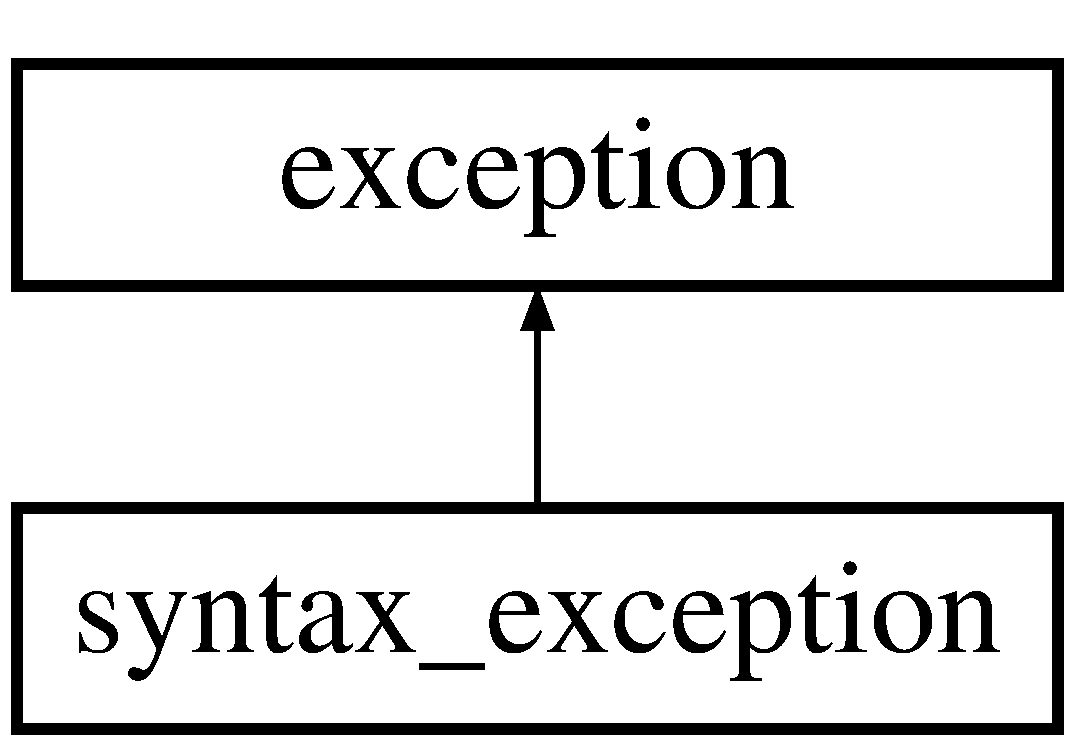
\includegraphics[height=2.000000cm]{classsyntax__exception}
\end{center}
\end{figure}
\subsection*{Public Member Functions}
\begin{DoxyCompactItemize}
\item 
\hyperlink{classsyntax__exception_a60278cf3cd3eba72c35f27ee36a21d68}{syntax\+\_\+exception} ()
\begin{DoxyCompactList}\small\item\em Default exeption constructor. \end{DoxyCompactList}\item 
\hyperlink{classsyntax__exception_aff5164bb18c155255820187afa2215c9}{syntax\+\_\+exception} (const std\+::string \&detail, size\+\_\+t line=(size\+\_\+t) -\/1)
\begin{DoxyCompactList}\small\item\em Exception constructor. \end{DoxyCompactList}\item 
const char $\ast$ \hyperlink{classsyntax__exception_a2a32f5e0c2acbbf37c10c9aa3d72506c}{what} () const  throw ()
\begin{DoxyCompactList}\small\item\em Tell what happened. \end{DoxyCompactList}\item 
size\+\_\+t \hyperlink{classsyntax__exception_aa25100b3e6601bb67aa5a5d1e76f508e}{getline} () const  throw ()
\begin{DoxyCompactList}\small\item\em Tell where it happened. \end{DoxyCompactList}\end{DoxyCompactItemize}


\subsection{Detailed Description}
Config class. 

This class defines I/O from/to a confi. file and handle differents exeptions.

Exception class for file parsing syntax errors. 

Definition at line 29 of file config\+\_\+load.\+h.



\subsection{Constructor \& Destructor Documentation}
\hypertarget{classsyntax__exception_a60278cf3cd3eba72c35f27ee36a21d68}{}\label{classsyntax__exception_a60278cf3cd3eba72c35f27ee36a21d68} 
\index{syntax\+\_\+exception@{syntax\+\_\+exception}!syntax\+\_\+exception@{syntax\+\_\+exception}}
\index{syntax\+\_\+exception@{syntax\+\_\+exception}!syntax\+\_\+exception@{syntax\+\_\+exception}}
\subsubsection{\texorpdfstring{syntax\+\_\+exception()}{syntax\_exception()}\hspace{0.1cm}{\footnotesize\ttfamily [1/2]}}
{\footnotesize\ttfamily syntax\+\_\+exception\+::syntax\+\_\+exception (\begin{DoxyParamCaption}{ }\end{DoxyParamCaption})}



Default exeption constructor. 



Definition at line 7 of file config\+\_\+load.\+cpp.

\hypertarget{classsyntax__exception_aff5164bb18c155255820187afa2215c9}{}\label{classsyntax__exception_aff5164bb18c155255820187afa2215c9} 
\index{syntax\+\_\+exception@{syntax\+\_\+exception}!syntax\+\_\+exception@{syntax\+\_\+exception}}
\index{syntax\+\_\+exception@{syntax\+\_\+exception}!syntax\+\_\+exception@{syntax\+\_\+exception}}
\subsubsection{\texorpdfstring{syntax\+\_\+exception()}{syntax\_exception()}\hspace{0.1cm}{\footnotesize\ttfamily [2/2]}}
{\footnotesize\ttfamily syntax\+\_\+exception\+::syntax\+\_\+exception (\begin{DoxyParamCaption}\item[{const std\+::string \&}]{detail,  }\item[{size\+\_\+t}]{line = {\ttfamily (size\+\_\+t)-\/1} }\end{DoxyParamCaption})}



Exception constructor. 

To create an exception message. A line can be specify if needed.


\begin{DoxyParams}{Parameters}
{\em line} & \+: Line where the exception as been lauched \\
\hline
{\em detail} & \+: Exception message \\
\hline
\end{DoxyParams}


Definition at line 11 of file config\+\_\+load.\+cpp.



\subsection{Member Function Documentation}
\hypertarget{classsyntax__exception_aa25100b3e6601bb67aa5a5d1e76f508e}{}\label{classsyntax__exception_aa25100b3e6601bb67aa5a5d1e76f508e} 
\index{syntax\+\_\+exception@{syntax\+\_\+exception}!getline@{getline}}
\index{getline@{getline}!syntax\+\_\+exception@{syntax\+\_\+exception}}
\subsubsection{\texorpdfstring{getline()}{getline()}}
{\footnotesize\ttfamily size\+\_\+t syntax\+\_\+exception\+::getline (\begin{DoxyParamCaption}{ }\end{DoxyParamCaption}) const throw  ) }



Tell where it happened. 

\begin{DoxyReturn}{Returns}
The line where error occurred 
\end{DoxyReturn}


Definition at line 20 of file config\+\_\+load.\+cpp.

\hypertarget{classsyntax__exception_a2a32f5e0c2acbbf37c10c9aa3d72506c}{}\label{classsyntax__exception_a2a32f5e0c2acbbf37c10c9aa3d72506c} 
\index{syntax\+\_\+exception@{syntax\+\_\+exception}!what@{what}}
\index{what@{what}!syntax\+\_\+exception@{syntax\+\_\+exception}}
\subsubsection{\texorpdfstring{what()}{what()}}
{\footnotesize\ttfamily const char $\ast$ syntax\+\_\+exception\+::what (\begin{DoxyParamCaption}{ }\end{DoxyParamCaption}) const throw  ) }



Tell what happened. 

If those functions throw an exception, something has gone horribly wrong !

\begin{DoxyReturn}{Returns}
A C string that contain the error message 
\end{DoxyReturn}


Definition at line 16 of file config\+\_\+load.\+cpp.



The documentation for this class was generated from the following files\+:\begin{DoxyCompactItemize}
\item 
\hyperlink{config__load_8h}{config\+\_\+load.\+h}\item 
\hyperlink{config__load_8cpp}{config\+\_\+load.\+cpp}\end{DoxyCompactItemize}

\chapter{File Documentation}
\hypertarget{board_8cpp}{}\section{board.\+cpp File Reference}
\label{board_8cpp}\index{board.\+cpp@{board.\+cpp}}
{\ttfamily \#include \char`\"{}board.\+h\char`\"{}}\newline
{\ttfamily \#include \char`\"{}config\+\_\+load.\+h\char`\"{}}\newline

\hypertarget{board_8h}{}\section{board.\+h File Reference}
\label{board_8h}\index{board.\+h@{board.\+h}}
{\ttfamily \#include \char`\"{}color.\+h\char`\"{}}\newline
{\ttfamily \#include \char`\"{}form.\+h\char`\"{}}\newline
{\ttfamily \#include $<$cstddef$>$}\newline
{\ttfamily \#include $<$string$>$}\newline
\subsection*{Classes}
\begin{DoxyCompactItemize}
\item 
class \hyperlink{class_board}{Board}
\begin{DoxyCompactList}\small\item\em \hyperlink{class_board}{Board} class. \end{DoxyCompactList}\end{DoxyCompactItemize}

\hypertarget{color_8cpp}{}\section{color.\+cpp File Reference}
\label{color_8cpp}\index{color.\+cpp@{color.\+cpp}}
{\ttfamily \#include \char`\"{}color.\+h\char`\"{}}\newline
\subsection*{Functions}
\begin{DoxyCompactItemize}
\item 
void \hyperlink{color_8cpp_acddb42733c81d53614791c18eae8fc30}{init\+\_\+color\+\_\+pairs} ()
\begin{DoxyCompactList}\small\item\em required by ncurse \end{DoxyCompactList}\item 
int \hyperlink{color_8cpp_ab3155e393c55030c30f44028f428ec5a}{get\+\_\+attr\+\_\+color} (int color)
\end{DoxyCompactItemize}


\subsection{Function Documentation}
\hypertarget{color_8cpp_ab3155e393c55030c30f44028f428ec5a}{}\label{color_8cpp_ab3155e393c55030c30f44028f428ec5a} 
\index{color.\+cpp@{color.\+cpp}!get\+\_\+attr\+\_\+color@{get\+\_\+attr\+\_\+color}}
\index{get\+\_\+attr\+\_\+color@{get\+\_\+attr\+\_\+color}!color.\+cpp@{color.\+cpp}}
\subsubsection{\texorpdfstring{get\+\_\+attr\+\_\+color()}{get\_attr\_color()}}
{\footnotesize\ttfamily int get\+\_\+attr\+\_\+color (\begin{DoxyParamCaption}\item[{int}]{color }\end{DoxyParamCaption})}



Definition at line 19 of file color.\+cpp.

\hypertarget{color_8cpp_acddb42733c81d53614791c18eae8fc30}{}\label{color_8cpp_acddb42733c81d53614791c18eae8fc30} 
\index{color.\+cpp@{color.\+cpp}!init\+\_\+color\+\_\+pairs@{init\+\_\+color\+\_\+pairs}}
\index{init\+\_\+color\+\_\+pairs@{init\+\_\+color\+\_\+pairs}!color.\+cpp@{color.\+cpp}}
\subsubsection{\texorpdfstring{init\+\_\+color\+\_\+pairs()}{init\_color\_pairs()}}
{\footnotesize\ttfamily void init\+\_\+color\+\_\+pairs (\begin{DoxyParamCaption}{ }\end{DoxyParamCaption})}



required by ncurse 



Definition at line 3 of file color.\+cpp.


\hypertarget{color_8h}{}\section{color.\+h File Reference}
\label{color_8h}\index{color.\+h@{color.\+h}}
{\ttfamily \#include $<$ncurses.\+h$>$}\newline
\subsection*{Macros}
\begin{DoxyCompactItemize}
\item 
\#define \hyperlink{color_8h_a4a87cda90141a2c984921221701de0ab}{C\+O\+L\+O\+R\+\_\+\+N\+O\+NE}~C\+O\+L\+O\+R\+\_\+\+B\+L\+A\+CK
\end{DoxyCompactItemize}
\subsection*{Enumerations}
\begin{DoxyCompactItemize}
\item 
enum \hyperlink{color_8h_a0b76cd27466f7debd3c57a4ae9585a84}{color\+Pair} \{ \newline
\hyperlink{color_8h_a0b76cd27466f7debd3c57a4ae9585a84a0af22a3a9b235e0ad0d159d3284b18bf}{D\+E\+F\+A\+U\+L\+T\+\_\+\+P\+A\+IR}, 
\hyperlink{color_8h_a0b76cd27466f7debd3c57a4ae9585a84ad4d53b59914a536f06a87a7a8a694231}{B\+L\+A\+C\+K\+\_\+\+R\+ED}, 
\hyperlink{color_8h_a0b76cd27466f7debd3c57a4ae9585a84a563bf8b94b8cb623fd9d17a6511cbad2}{B\+L\+A\+C\+K\+\_\+\+G\+R\+E\+EN}, 
\hyperlink{color_8h_a0b76cd27466f7debd3c57a4ae9585a84a69c6d074dde26482b93bc29242d2044c}{B\+L\+A\+C\+K\+\_\+\+Y\+E\+L\+L\+OW}, 
\newline
\hyperlink{color_8h_a0b76cd27466f7debd3c57a4ae9585a84a7ea9008e5111c16cd317d8daffe21f0a}{B\+L\+A\+C\+K\+\_\+\+B\+L\+UE}, 
\hyperlink{color_8h_a0b76cd27466f7debd3c57a4ae9585a84ae582c733b432f64138d32ecf8654d710}{B\+L\+A\+C\+K\+\_\+\+M\+A\+G\+E\+N\+TA}, 
\hyperlink{color_8h_a0b76cd27466f7debd3c57a4ae9585a84a6891812b72fa1cd39e359d7f8539c9b7}{B\+L\+A\+C\+K\+\_\+\+C\+Y\+AN}, 
\hyperlink{color_8h_a0b76cd27466f7debd3c57a4ae9585a84a2879550cb7b282e89baaddb83f921d73}{B\+L\+A\+C\+K\+\_\+\+W\+H\+I\+TE}, 
\newline
\hyperlink{color_8h_a0b76cd27466f7debd3c57a4ae9585a84a8eb80d1f88b31998106932eba9a21029}{R\+E\+D\+\_\+\+B\+L\+A\+CK}, 
\hyperlink{color_8h_a0b76cd27466f7debd3c57a4ae9585a84a189a7800234e077b2d997d65da120818}{B\+L\+U\+E\+\_\+\+B\+L\+A\+CK}, 
\hyperlink{color_8h_a0b76cd27466f7debd3c57a4ae9585a84a07aa836826cf14afc4e9af0c7df630eb}{Y\+E\+L\+L\+O\+W\+\_\+\+B\+L\+A\+CK}, 
\hyperlink{color_8h_a0b76cd27466f7debd3c57a4ae9585a84a6d961e34f5bdac161d0cb023818a85d3}{M\+A\+X\+\_\+\+P\+A\+IR}
 \}\begin{DoxyCompactList}\small\item\em Colors pairs. \end{DoxyCompactList}
\end{DoxyCompactItemize}
\subsection*{Functions}
\begin{DoxyCompactItemize}
\item 
void \hyperlink{color_8h_acddb42733c81d53614791c18eae8fc30}{init\+\_\+color\+\_\+pairs} ()
\begin{DoxyCompactList}\small\item\em required by ncurse \end{DoxyCompactList}\item 
int \hyperlink{color_8h_a77e9f82ef1751b8e2d6eb9fee5e0ff47}{get\+\_\+attr\+\_\+color} (int)
\end{DoxyCompactItemize}


\subsection{Macro Definition Documentation}
\hypertarget{color_8h_a4a87cda90141a2c984921221701de0ab}{}\label{color_8h_a4a87cda90141a2c984921221701de0ab} 
\index{color.\+h@{color.\+h}!C\+O\+L\+O\+R\+\_\+\+N\+O\+NE@{C\+O\+L\+O\+R\+\_\+\+N\+O\+NE}}
\index{C\+O\+L\+O\+R\+\_\+\+N\+O\+NE@{C\+O\+L\+O\+R\+\_\+\+N\+O\+NE}!color.\+h@{color.\+h}}
\subsubsection{\texorpdfstring{C\+O\+L\+O\+R\+\_\+\+N\+O\+NE}{COLOR\_NONE}}
{\footnotesize\ttfamily \#define C\+O\+L\+O\+R\+\_\+\+N\+O\+NE~C\+O\+L\+O\+R\+\_\+\+B\+L\+A\+CK}



Definition at line 19 of file color.\+h.



\subsection{Enumeration Type Documentation}
\hypertarget{color_8h_a0b76cd27466f7debd3c57a4ae9585a84}{}\label{color_8h_a0b76cd27466f7debd3c57a4ae9585a84} 
\index{color.\+h@{color.\+h}!color\+Pair@{color\+Pair}}
\index{color\+Pair@{color\+Pair}!color.\+h@{color.\+h}}
\subsubsection{\texorpdfstring{color\+Pair}{colorPair}}
{\footnotesize\ttfamily enum \hyperlink{color_8h_a0b76cd27466f7debd3c57a4ae9585a84}{color\+Pair}}



Colors pairs. 

Create all macro required by ncurse to describe colors. Every square\textquotesingle{}s color in the grid is define by a pair with blanck caracter writed on a colord backfont. Color pair 0 is reserved by ncurses as default color pair it is initialized by start\+\_\+colors() and should not be modified. \begin{DoxyEnumFields}{Enumerator}
\raisebox{\heightof{T}}[0pt][0pt]{\index{D\+E\+F\+A\+U\+L\+T\+\_\+\+P\+A\+IR@{D\+E\+F\+A\+U\+L\+T\+\_\+\+P\+A\+IR}!color.\+h@{color.\+h}}\index{color.\+h@{color.\+h}!D\+E\+F\+A\+U\+L\+T\+\_\+\+P\+A\+IR@{D\+E\+F\+A\+U\+L\+T\+\_\+\+P\+A\+IR}}}\hypertarget{color_8h_a0b76cd27466f7debd3c57a4ae9585a84a0af22a3a9b235e0ad0d159d3284b18bf}{}\label{color_8h_a0b76cd27466f7debd3c57a4ae9585a84a0af22a3a9b235e0ad0d159d3284b18bf} 
D\+E\+F\+A\+U\+L\+T\+\_\+\+P\+A\+IR&Default pair. \\
\hline

\raisebox{\heightof{T}}[0pt][0pt]{\index{B\+L\+A\+C\+K\+\_\+\+R\+ED@{B\+L\+A\+C\+K\+\_\+\+R\+ED}!color.\+h@{color.\+h}}\index{color.\+h@{color.\+h}!B\+L\+A\+C\+K\+\_\+\+R\+ED@{B\+L\+A\+C\+K\+\_\+\+R\+ED}}}\hypertarget{color_8h_a0b76cd27466f7debd3c57a4ae9585a84ad4d53b59914a536f06a87a7a8a694231}{}\label{color_8h_a0b76cd27466f7debd3c57a4ae9585a84ad4d53b59914a536f06a87a7a8a694231} 
B\+L\+A\+C\+K\+\_\+\+R\+ED&Red square. \\
\hline

\raisebox{\heightof{T}}[0pt][0pt]{\index{B\+L\+A\+C\+K\+\_\+\+G\+R\+E\+EN@{B\+L\+A\+C\+K\+\_\+\+G\+R\+E\+EN}!color.\+h@{color.\+h}}\index{color.\+h@{color.\+h}!B\+L\+A\+C\+K\+\_\+\+G\+R\+E\+EN@{B\+L\+A\+C\+K\+\_\+\+G\+R\+E\+EN}}}\hypertarget{color_8h_a0b76cd27466f7debd3c57a4ae9585a84a563bf8b94b8cb623fd9d17a6511cbad2}{}\label{color_8h_a0b76cd27466f7debd3c57a4ae9585a84a563bf8b94b8cb623fd9d17a6511cbad2} 
B\+L\+A\+C\+K\+\_\+\+G\+R\+E\+EN&Green square. \\
\hline

\raisebox{\heightof{T}}[0pt][0pt]{\index{B\+L\+A\+C\+K\+\_\+\+Y\+E\+L\+L\+OW@{B\+L\+A\+C\+K\+\_\+\+Y\+E\+L\+L\+OW}!color.\+h@{color.\+h}}\index{color.\+h@{color.\+h}!B\+L\+A\+C\+K\+\_\+\+Y\+E\+L\+L\+OW@{B\+L\+A\+C\+K\+\_\+\+Y\+E\+L\+L\+OW}}}\hypertarget{color_8h_a0b76cd27466f7debd3c57a4ae9585a84a69c6d074dde26482b93bc29242d2044c}{}\label{color_8h_a0b76cd27466f7debd3c57a4ae9585a84a69c6d074dde26482b93bc29242d2044c} 
B\+L\+A\+C\+K\+\_\+\+Y\+E\+L\+L\+OW&Yellow square. \\
\hline

\raisebox{\heightof{T}}[0pt][0pt]{\index{B\+L\+A\+C\+K\+\_\+\+B\+L\+UE@{B\+L\+A\+C\+K\+\_\+\+B\+L\+UE}!color.\+h@{color.\+h}}\index{color.\+h@{color.\+h}!B\+L\+A\+C\+K\+\_\+\+B\+L\+UE@{B\+L\+A\+C\+K\+\_\+\+B\+L\+UE}}}\hypertarget{color_8h_a0b76cd27466f7debd3c57a4ae9585a84a7ea9008e5111c16cd317d8daffe21f0a}{}\label{color_8h_a0b76cd27466f7debd3c57a4ae9585a84a7ea9008e5111c16cd317d8daffe21f0a} 
B\+L\+A\+C\+K\+\_\+\+B\+L\+UE&Blue square. \\
\hline

\raisebox{\heightof{T}}[0pt][0pt]{\index{B\+L\+A\+C\+K\+\_\+\+M\+A\+G\+E\+N\+TA@{B\+L\+A\+C\+K\+\_\+\+M\+A\+G\+E\+N\+TA}!color.\+h@{color.\+h}}\index{color.\+h@{color.\+h}!B\+L\+A\+C\+K\+\_\+\+M\+A\+G\+E\+N\+TA@{B\+L\+A\+C\+K\+\_\+\+M\+A\+G\+E\+N\+TA}}}\hypertarget{color_8h_a0b76cd27466f7debd3c57a4ae9585a84ae582c733b432f64138d32ecf8654d710}{}\label{color_8h_a0b76cd27466f7debd3c57a4ae9585a84ae582c733b432f64138d32ecf8654d710} 
B\+L\+A\+C\+K\+\_\+\+M\+A\+G\+E\+N\+TA&Magenta square. \\
\hline

\raisebox{\heightof{T}}[0pt][0pt]{\index{B\+L\+A\+C\+K\+\_\+\+C\+Y\+AN@{B\+L\+A\+C\+K\+\_\+\+C\+Y\+AN}!color.\+h@{color.\+h}}\index{color.\+h@{color.\+h}!B\+L\+A\+C\+K\+\_\+\+C\+Y\+AN@{B\+L\+A\+C\+K\+\_\+\+C\+Y\+AN}}}\hypertarget{color_8h_a0b76cd27466f7debd3c57a4ae9585a84a6891812b72fa1cd39e359d7f8539c9b7}{}\label{color_8h_a0b76cd27466f7debd3c57a4ae9585a84a6891812b72fa1cd39e359d7f8539c9b7} 
B\+L\+A\+C\+K\+\_\+\+C\+Y\+AN&Cyan square. \\
\hline

\raisebox{\heightof{T}}[0pt][0pt]{\index{B\+L\+A\+C\+K\+\_\+\+W\+H\+I\+TE@{B\+L\+A\+C\+K\+\_\+\+W\+H\+I\+TE}!color.\+h@{color.\+h}}\index{color.\+h@{color.\+h}!B\+L\+A\+C\+K\+\_\+\+W\+H\+I\+TE@{B\+L\+A\+C\+K\+\_\+\+W\+H\+I\+TE}}}\hypertarget{color_8h_a0b76cd27466f7debd3c57a4ae9585a84a2879550cb7b282e89baaddb83f921d73}{}\label{color_8h_a0b76cd27466f7debd3c57a4ae9585a84a2879550cb7b282e89baaddb83f921d73} 
B\+L\+A\+C\+K\+\_\+\+W\+H\+I\+TE&White square. \\
\hline

\raisebox{\heightof{T}}[0pt][0pt]{\index{R\+E\+D\+\_\+\+B\+L\+A\+CK@{R\+E\+D\+\_\+\+B\+L\+A\+CK}!color.\+h@{color.\+h}}\index{color.\+h@{color.\+h}!R\+E\+D\+\_\+\+B\+L\+A\+CK@{R\+E\+D\+\_\+\+B\+L\+A\+CK}}}\hypertarget{color_8h_a0b76cd27466f7debd3c57a4ae9585a84a8eb80d1f88b31998106932eba9a21029}{}\label{color_8h_a0b76cd27466f7debd3c57a4ae9585a84a8eb80d1f88b31998106932eba9a21029} 
R\+E\+D\+\_\+\+B\+L\+A\+CK&Red font. \\
\hline

\raisebox{\heightof{T}}[0pt][0pt]{\index{B\+L\+U\+E\+\_\+\+B\+L\+A\+CK@{B\+L\+U\+E\+\_\+\+B\+L\+A\+CK}!color.\+h@{color.\+h}}\index{color.\+h@{color.\+h}!B\+L\+U\+E\+\_\+\+B\+L\+A\+CK@{B\+L\+U\+E\+\_\+\+B\+L\+A\+CK}}}\hypertarget{color_8h_a0b76cd27466f7debd3c57a4ae9585a84a189a7800234e077b2d997d65da120818}{}\label{color_8h_a0b76cd27466f7debd3c57a4ae9585a84a189a7800234e077b2d997d65da120818} 
B\+L\+U\+E\+\_\+\+B\+L\+A\+CK&Blue font. \\
\hline

\raisebox{\heightof{T}}[0pt][0pt]{\index{Y\+E\+L\+L\+O\+W\+\_\+\+B\+L\+A\+CK@{Y\+E\+L\+L\+O\+W\+\_\+\+B\+L\+A\+CK}!color.\+h@{color.\+h}}\index{color.\+h@{color.\+h}!Y\+E\+L\+L\+O\+W\+\_\+\+B\+L\+A\+CK@{Y\+E\+L\+L\+O\+W\+\_\+\+B\+L\+A\+CK}}}\hypertarget{color_8h_a0b76cd27466f7debd3c57a4ae9585a84a07aa836826cf14afc4e9af0c7df630eb}{}\label{color_8h_a0b76cd27466f7debd3c57a4ae9585a84a07aa836826cf14afc4e9af0c7df630eb} 
Y\+E\+L\+L\+O\+W\+\_\+\+B\+L\+A\+CK&Yellow font. \\
\hline

\raisebox{\heightof{T}}[0pt][0pt]{\index{M\+A\+X\+\_\+\+P\+A\+IR@{M\+A\+X\+\_\+\+P\+A\+IR}!color.\+h@{color.\+h}}\index{color.\+h@{color.\+h}!M\+A\+X\+\_\+\+P\+A\+IR@{M\+A\+X\+\_\+\+P\+A\+IR}}}\hypertarget{color_8h_a0b76cd27466f7debd3c57a4ae9585a84a6d961e34f5bdac161d0cb023818a85d3}{}\label{color_8h_a0b76cd27466f7debd3c57a4ae9585a84a6d961e34f5bdac161d0cb023818a85d3} 
M\+A\+X\+\_\+\+P\+A\+IR&Number of pairs defined. \\
\hline

\end{DoxyEnumFields}


Definition at line 30 of file color.\+h.



\subsection{Function Documentation}
\hypertarget{color_8h_a77e9f82ef1751b8e2d6eb9fee5e0ff47}{}\label{color_8h_a77e9f82ef1751b8e2d6eb9fee5e0ff47} 
\index{color.\+h@{color.\+h}!get\+\_\+attr\+\_\+color@{get\+\_\+attr\+\_\+color}}
\index{get\+\_\+attr\+\_\+color@{get\+\_\+attr\+\_\+color}!color.\+h@{color.\+h}}
\subsubsection{\texorpdfstring{get\+\_\+attr\+\_\+color()}{get\_attr\_color()}}
{\footnotesize\ttfamily int get\+\_\+attr\+\_\+color (\begin{DoxyParamCaption}\item[{int}]{ }\end{DoxyParamCaption})}



Definition at line 19 of file color.\+cpp.

\hypertarget{color_8h_acddb42733c81d53614791c18eae8fc30}{}\label{color_8h_acddb42733c81d53614791c18eae8fc30} 
\index{color.\+h@{color.\+h}!init\+\_\+color\+\_\+pairs@{init\+\_\+color\+\_\+pairs}}
\index{init\+\_\+color\+\_\+pairs@{init\+\_\+color\+\_\+pairs}!color.\+h@{color.\+h}}
\subsubsection{\texorpdfstring{init\+\_\+color\+\_\+pairs()}{init\_color\_pairs()}}
{\footnotesize\ttfamily void init\+\_\+color\+\_\+pairs (\begin{DoxyParamCaption}{ }\end{DoxyParamCaption})}



required by ncurse 



Definition at line 3 of file color.\+cpp.


\hypertarget{config__load_8cpp}{}\section{config\+\_\+load.\+cpp File Reference}
\label{config__load_8cpp}\index{config\+\_\+load.\+cpp@{config\+\_\+load.\+cpp}}
{\ttfamily \#include \char`\"{}config\+\_\+load.\+h\char`\"{}}\newline
{\ttfamily \#include \char`\"{}color.\+h\char`\"{}}\newline
{\ttfamily \#include \char`\"{}global\+\_\+log.\+h\char`\"{}}\newline
\subsection*{Functions}
\begin{DoxyCompactItemize}
\item 
bool \hyperlink{config__load_8cpp_a636244d246012f87b5003695c2e7087e}{blank\+\_\+only} (const std\+::string \&str)
\begin{DoxyCompactList}\small\item\em Check if a the string contain only blanck caracters. \end{DoxyCompactList}\item 
size\+\_\+t \hyperlink{config__load_8cpp_abc3153a083a56debb6ae2110d5d519ad}{count\+\_\+occurences} (const std\+::string \&input, const std\+::string \&ch)
\begin{DoxyCompactList}\small\item\em Count occurences of any of the characters in a string. \end{DoxyCompactList}\item 
size\+\_\+t \hyperlink{config__load_8cpp_a0b3d65604cb86fecc02a99a3a2235c81}{count\+\_\+occurences} (const std\+::string \&input, const char $\ast$ch)
\begin{DoxyCompactList}\small\item\em Count occurences of any of the characters in a string. \end{DoxyCompactList}\item 
size\+\_\+t \hyperlink{config__load_8cpp_aa13750b8e0385d9be2128e99355f0e98}{count\+\_\+occurences} (const std\+::string \&input, const char $\ast$ch, size\+\_\+t n)
\begin{DoxyCompactList}\small\item\em Count occurences of any of the characters in a string. \end{DoxyCompactList}\item 
size\+\_\+t \hyperlink{config__load_8cpp_a899ade67be61798ffcf05b9e76cf2ab7}{count\+\_\+occurences} (const std\+::string \&input, char ch)
\begin{DoxyCompactList}\small\item\em Count occurences of any of the characters in a string. \end{DoxyCompactList}\item 
void \hyperlink{config__load_8cpp_ade1b6c26e93a6e2d06d517638b4f9ef8}{clean\+\_\+config\+\_\+input} (std\+::string \&input)
\begin{DoxyCompactList}\small\item\em Standard config input cleaning function. \end{DoxyCompactList}\item 
std\+::string \hyperlink{config__load_8cpp_aa1b160b86794a8c3423085fabd7f9d4f}{getword} (std\+::string \&input)
\begin{DoxyCompactList}\small\item\em Get a word at the begining of a string then remove it. \end{DoxyCompactList}\item 
std\+::string \hyperlink{config__load_8cpp_a0aec8604cf53ec108542fbb2edbf48f0}{getline} (std\+::string \&input)
\begin{DoxyCompactList}\small\item\em Get a line at the begining of a string then remove it. \end{DoxyCompactList}\item 
std\+::string \hyperlink{config__load_8cpp_a6572cd7b7c7694d505d449783ad09816}{getblock} (std\+::string \&input, size\+\_\+t $\ast$line)
\begin{DoxyCompactList}\small\item\em Get a block between \textquotesingle{}\{\textquotesingle{} and \textquotesingle{}\}\textquotesingle{}. \end{DoxyCompactList}\item 
bool \hyperlink{config__load_8cpp_ae85e3061deff8801e70fa840a7ff23a2}{get\+\_\+key\+\_\+value} (const std\+::string \&input, std\+::string \&key, std\+::string \&value)
\begin{DoxyCompactList}\small\item\em Search a title. \end{DoxyCompactList}\item 
void \hyperlink{config__load_8cpp_ac644b36db96f2c826276a4a772227faa}{set\+\_\+case} (std\+::string \&str, bool lower)
\begin{DoxyCompactList}\small\item\em Convert a string to all U\+P\+P\+ER / lower case. \end{DoxyCompactList}\item 
int \hyperlink{config__load_8cpp_ad8b2e1b1979839c9c2ad2397aea3f331}{word\+\_\+to\+\_\+color} (const std\+::string \&input)
\item 
std\+::string \hyperlink{config__load_8cpp_a184b1d81e1b38c7d069379acc85a4c60}{color\+\_\+to\+\_\+word} (int color)
\begin{DoxyCompactList}\small\item\em Convert a color code to its corresponding name. \end{DoxyCompactList}\end{DoxyCompactItemize}


\subsection{Function Documentation}
\hypertarget{config__load_8cpp_a636244d246012f87b5003695c2e7087e}{}\label{config__load_8cpp_a636244d246012f87b5003695c2e7087e} 
\index{config\+\_\+load.\+cpp@{config\+\_\+load.\+cpp}!blank\+\_\+only@{blank\+\_\+only}}
\index{blank\+\_\+only@{blank\+\_\+only}!config\+\_\+load.\+cpp@{config\+\_\+load.\+cpp}}
\subsubsection{\texorpdfstring{blank\+\_\+only()}{blank\_only()}}
{\footnotesize\ttfamily bool blank\+\_\+only (\begin{DoxyParamCaption}\item[{const std\+::string \&}]{ }\end{DoxyParamCaption})}



Check if a the string contain only blanck caracters. 

\begin{DoxyReturn}{Returns}
true if string contain only spaces, tabs and newlines 
\end{DoxyReturn}


Definition at line 25 of file config\+\_\+load.\+cpp.

\hypertarget{config__load_8cpp_ade1b6c26e93a6e2d06d517638b4f9ef8}{}\label{config__load_8cpp_ade1b6c26e93a6e2d06d517638b4f9ef8} 
\index{config\+\_\+load.\+cpp@{config\+\_\+load.\+cpp}!clean\+\_\+config\+\_\+input@{clean\+\_\+config\+\_\+input}}
\index{clean\+\_\+config\+\_\+input@{clean\+\_\+config\+\_\+input}!config\+\_\+load.\+cpp@{config\+\_\+load.\+cpp}}
\subsubsection{\texorpdfstring{clean\+\_\+config\+\_\+input()}{clean\_config\_input()}}
{\footnotesize\ttfamily void clean\+\_\+config\+\_\+input (\begin{DoxyParamCaption}\item[{std\+::string \&}]{input }\end{DoxyParamCaption})}



Standard config input cleaning function. 

Remove blank (space, tab and newline) at the begining and the end. Then replace any sequence of blank by a single space


\begin{DoxyParams}{Parameters}
{\em input} & \+: The string to clean \\
\hline
\end{DoxyParams}


Definition at line 71 of file config\+\_\+load.\+cpp.

\hypertarget{config__load_8cpp_a184b1d81e1b38c7d069379acc85a4c60}{}\label{config__load_8cpp_a184b1d81e1b38c7d069379acc85a4c60} 
\index{config\+\_\+load.\+cpp@{config\+\_\+load.\+cpp}!color\+\_\+to\+\_\+word@{color\+\_\+to\+\_\+word}}
\index{color\+\_\+to\+\_\+word@{color\+\_\+to\+\_\+word}!config\+\_\+load.\+cpp@{config\+\_\+load.\+cpp}}
\subsubsection{\texorpdfstring{color\+\_\+to\+\_\+word()}{color\_to\_word()}}
{\footnotesize\ttfamily std\+::string color\+\_\+to\+\_\+word (\begin{DoxyParamCaption}\item[{int}]{code }\end{DoxyParamCaption})}



Convert a color code to its corresponding name. 

Color names will be one following \+: B\+L\+A\+CK, R\+ED, G\+R\+E\+EN, Y\+E\+L\+L\+OW, B\+L\+UE, M\+A\+G\+E\+N\+TA, C\+Y\+AN, W\+H\+I\+TE.


\begin{DoxyParams}{Parameters}
{\em code} & \+: The color\textquotesingle{}s code\\
\hline
\end{DoxyParams}
\begin{DoxyReturn}{Returns}
The color\textquotesingle{}s corresponding name 
\end{DoxyReturn}


Definition at line 217 of file config\+\_\+load.\+cpp.

\hypertarget{config__load_8cpp_abc3153a083a56debb6ae2110d5d519ad}{}\label{config__load_8cpp_abc3153a083a56debb6ae2110d5d519ad} 
\index{config\+\_\+load.\+cpp@{config\+\_\+load.\+cpp}!count\+\_\+occurences@{count\+\_\+occurences}}
\index{count\+\_\+occurences@{count\+\_\+occurences}!config\+\_\+load.\+cpp@{config\+\_\+load.\+cpp}}
\subsubsection{\texorpdfstring{count\+\_\+occurences()}{count\_occurences()}\hspace{0.1cm}{\footnotesize\ttfamily [1/4]}}
{\footnotesize\ttfamily size\+\_\+t count\+\_\+occurences (\begin{DoxyParamCaption}\item[{const std\+::string \&}]{input,  }\item[{const std\+::string \&}]{ch }\end{DoxyParamCaption})}



Count occurences of any of the characters in a string. 

Character set (second argument) is passed as in string\+::find\+\_\+first\+\_\+of()


\begin{DoxyParams}{Parameters}
{\em input} & \+: The string where to search \\
\hline
{\em ch} & \+: The caracter to search\\
\hline
\end{DoxyParams}
\begin{DoxyReturn}{Returns}
Number of occurences 
\end{DoxyReturn}


Definition at line 30 of file config\+\_\+load.\+cpp.

\hypertarget{config__load_8cpp_a0b3d65604cb86fecc02a99a3a2235c81}{}\label{config__load_8cpp_a0b3d65604cb86fecc02a99a3a2235c81} 
\index{config\+\_\+load.\+cpp@{config\+\_\+load.\+cpp}!count\+\_\+occurences@{count\+\_\+occurences}}
\index{count\+\_\+occurences@{count\+\_\+occurences}!config\+\_\+load.\+cpp@{config\+\_\+load.\+cpp}}
\subsubsection{\texorpdfstring{count\+\_\+occurences()}{count\_occurences()}\hspace{0.1cm}{\footnotesize\ttfamily [2/4]}}
{\footnotesize\ttfamily size\+\_\+t count\+\_\+occurences (\begin{DoxyParamCaption}\item[{const std\+::string \&}]{input,  }\item[{const char $\ast$}]{ch }\end{DoxyParamCaption})}



Count occurences of any of the characters in a string. 

Character set (second argument) is passed as in string\+::find\+\_\+first\+\_\+of()


\begin{DoxyParams}{Parameters}
{\em input} & \+: The string where to search \\
\hline
{\em ch} & \+: The caracter to search\\
\hline
\end{DoxyParams}
\begin{DoxyReturn}{Returns}
Number of occurences 
\end{DoxyReturn}


Definition at line 40 of file config\+\_\+load.\+cpp.

\hypertarget{config__load_8cpp_aa13750b8e0385d9be2128e99355f0e98}{}\label{config__load_8cpp_aa13750b8e0385d9be2128e99355f0e98} 
\index{config\+\_\+load.\+cpp@{config\+\_\+load.\+cpp}!count\+\_\+occurences@{count\+\_\+occurences}}
\index{count\+\_\+occurences@{count\+\_\+occurences}!config\+\_\+load.\+cpp@{config\+\_\+load.\+cpp}}
\subsubsection{\texorpdfstring{count\+\_\+occurences()}{count\_occurences()}\hspace{0.1cm}{\footnotesize\ttfamily [3/4]}}
{\footnotesize\ttfamily size\+\_\+t count\+\_\+occurences (\begin{DoxyParamCaption}\item[{const std\+::string \&}]{input,  }\item[{const char $\ast$}]{ch,  }\item[{size\+\_\+t}]{ }\end{DoxyParamCaption})}



Count occurences of any of the characters in a string. 

Character set (second argument) is passed as in string\+::find\+\_\+first\+\_\+of()


\begin{DoxyParams}{Parameters}
{\em input} & \+: The string where to search \\
\hline
{\em ch} & \+: The caracter to search \\
\hline
{\em n} & \+: Number of character values to search for\\
\hline
\end{DoxyParams}
\begin{DoxyReturn}{Returns}
Number of occurences 
\end{DoxyReturn}


Definition at line 50 of file config\+\_\+load.\+cpp.

\hypertarget{config__load_8cpp_a899ade67be61798ffcf05b9e76cf2ab7}{}\label{config__load_8cpp_a899ade67be61798ffcf05b9e76cf2ab7} 
\index{config\+\_\+load.\+cpp@{config\+\_\+load.\+cpp}!count\+\_\+occurences@{count\+\_\+occurences}}
\index{count\+\_\+occurences@{count\+\_\+occurences}!config\+\_\+load.\+cpp@{config\+\_\+load.\+cpp}}
\subsubsection{\texorpdfstring{count\+\_\+occurences()}{count\_occurences()}\hspace{0.1cm}{\footnotesize\ttfamily [4/4]}}
{\footnotesize\ttfamily size\+\_\+t count\+\_\+occurences (\begin{DoxyParamCaption}\item[{const std\+::string \&}]{input,  }\item[{char}]{ch }\end{DoxyParamCaption})}



Count occurences of any of the characters in a string. 

Character set (second argument) is passed as in string\+::find\+\_\+first\+\_\+of()


\begin{DoxyParams}{Parameters}
{\em input} & \+: The string where to search \\
\hline
{\em ch} & \+: The caracter to search\\
\hline
\end{DoxyParams}
\begin{DoxyReturn}{Returns}
Number of occurences 
\end{DoxyReturn}


Definition at line 60 of file config\+\_\+load.\+cpp.

\hypertarget{config__load_8cpp_ae85e3061deff8801e70fa840a7ff23a2}{}\label{config__load_8cpp_ae85e3061deff8801e70fa840a7ff23a2} 
\index{config\+\_\+load.\+cpp@{config\+\_\+load.\+cpp}!get\+\_\+key\+\_\+value@{get\+\_\+key\+\_\+value}}
\index{get\+\_\+key\+\_\+value@{get\+\_\+key\+\_\+value}!config\+\_\+load.\+cpp@{config\+\_\+load.\+cpp}}
\subsubsection{\texorpdfstring{get\+\_\+key\+\_\+value()}{get\_key\_value()}}
{\footnotesize\ttfamily bool get\+\_\+key\+\_\+value (\begin{DoxyParamCaption}\item[{const std\+::string \&}]{input,  }\item[{std\+::string \&}]{key,  }\item[{std\+::string \&}]{value }\end{DoxyParamCaption})}



Search a title. 

Look for the sequence \char`\"{} \+: \char`\"{} in a string If the sequence is found, set key to the first part (before \+: ) and value to the second (after \+: ) and return true. If not, return false. If value is empty, second space is optional. Only the first \char`\"{} \+: \char`\"{} is considered.


\begin{DoxyParams}{Parameters}
{\em input} & \+: The string where search for the sequence \textquotesingle{}\+:\textquotesingle{} \\
\hline
{\em line} & \+: The keyword that describe the sequence find \\
\hline
{\em value} & \+: The sequence value\\
\hline
\end{DoxyParams}
\begin{DoxyReturn}{Returns}
True is the sequence has been found 
\end{DoxyReturn}


Definition at line 157 of file config\+\_\+load.\+cpp.

\hypertarget{config__load_8cpp_a6572cd7b7c7694d505d449783ad09816}{}\label{config__load_8cpp_a6572cd7b7c7694d505d449783ad09816} 
\index{config\+\_\+load.\+cpp@{config\+\_\+load.\+cpp}!getblock@{getblock}}
\index{getblock@{getblock}!config\+\_\+load.\+cpp@{config\+\_\+load.\+cpp}}
\subsubsection{\texorpdfstring{getblock()}{getblock()}}
{\footnotesize\ttfamily std\+::string getblock (\begin{DoxyParamCaption}\item[{std\+::string \&}]{input,  }\item[{size\+\_\+t $\ast$}]{line = {\ttfamily nullptr} }\end{DoxyParamCaption})}



Get a block between \textquotesingle{}\{\textquotesingle{} and \textquotesingle{}\}\textquotesingle{}. 

Before first \textquotesingle{}\{\textquotesingle{} shall only be blank. Return the block and remove it as well as \{ \} from input. Line is set to the number of lines removed from input


\begin{DoxyParams}{Parameters}
{\em input} & \+: The string where extract the block \\
\hline
{\em line} & \+: The number of line extracted (ie. block\textquotesingle{}s size)\\
\hline
\end{DoxyParams}
\begin{DoxyReturn}{Returns}
The block extracted 
\end{DoxyReturn}


Definition at line 123 of file config\+\_\+load.\+cpp.

\hypertarget{config__load_8cpp_a0aec8604cf53ec108542fbb2edbf48f0}{}\label{config__load_8cpp_a0aec8604cf53ec108542fbb2edbf48f0} 
\index{config\+\_\+load.\+cpp@{config\+\_\+load.\+cpp}!getline@{getline}}
\index{getline@{getline}!config\+\_\+load.\+cpp@{config\+\_\+load.\+cpp}}
\subsubsection{\texorpdfstring{getline()}{getline()}}
{\footnotesize\ttfamily std\+::string getline (\begin{DoxyParamCaption}\item[{std\+::string \&}]{ }\end{DoxyParamCaption})}



Get a line at the begining of a string then remove it. 


\begin{DoxyParams}{Parameters}
{\em input} & \+: The string where extract the 1st line\\
\hline
\end{DoxyParams}
\begin{DoxyReturn}{Returns}
The extracted line 
\end{DoxyReturn}


Definition at line 110 of file config\+\_\+load.\+cpp.

\hypertarget{config__load_8cpp_aa1b160b86794a8c3423085fabd7f9d4f}{}\label{config__load_8cpp_aa1b160b86794a8c3423085fabd7f9d4f} 
\index{config\+\_\+load.\+cpp@{config\+\_\+load.\+cpp}!getword@{getword}}
\index{getword@{getword}!config\+\_\+load.\+cpp@{config\+\_\+load.\+cpp}}
\subsubsection{\texorpdfstring{getword()}{getword()}}
{\footnotesize\ttfamily std\+::string getword (\begin{DoxyParamCaption}\item[{std\+::string \&}]{input }\end{DoxyParamCaption})}



Get a word at the begining of a string then remove it. 

A word is the group of caracters from begining to the first blank. The blank is removed as well, it is designed for use on string cleaned with clean\+\_\+config\+\_\+input.


\begin{DoxyParams}{Parameters}
{\em input} & \+: The string where extract the 1st word\\
\hline
\end{DoxyParams}
\begin{DoxyReturn}{Returns}
The extracted word 
\end{DoxyReturn}


Definition at line 97 of file config\+\_\+load.\+cpp.

\hypertarget{config__load_8cpp_ac644b36db96f2c826276a4a772227faa}{}\label{config__load_8cpp_ac644b36db96f2c826276a4a772227faa} 
\index{config\+\_\+load.\+cpp@{config\+\_\+load.\+cpp}!set\+\_\+case@{set\+\_\+case}}
\index{set\+\_\+case@{set\+\_\+case}!config\+\_\+load.\+cpp@{config\+\_\+load.\+cpp}}
\subsubsection{\texorpdfstring{set\+\_\+case()}{set\_case()}}
{\footnotesize\ttfamily void set\+\_\+case (\begin{DoxyParamCaption}\item[{std\+::string \&}]{str,  }\item[{bool}]{lower = {\ttfamily false} }\end{DoxyParamCaption})}



Convert a string to all U\+P\+P\+ER / lower case. 

By default it convert to lower.


\begin{DoxyParams}{Parameters}
{\em str} & \+: The string to convert \\
\hline
{\em lower} & \+: Case wanted \\
\hline
\end{DoxyParams}


Definition at line 179 of file config\+\_\+load.\+cpp.

\hypertarget{config__load_8cpp_ad8b2e1b1979839c9c2ad2397aea3f331}{}\label{config__load_8cpp_ad8b2e1b1979839c9c2ad2397aea3f331} 
\index{config\+\_\+load.\+cpp@{config\+\_\+load.\+cpp}!word\+\_\+to\+\_\+color@{word\+\_\+to\+\_\+color}}
\index{word\+\_\+to\+\_\+color@{word\+\_\+to\+\_\+color}!config\+\_\+load.\+cpp@{config\+\_\+load.\+cpp}}
\subsubsection{\texorpdfstring{word\+\_\+to\+\_\+color()}{word\_to\_color()}}
{\footnotesize\ttfamily int word\+\_\+to\+\_\+color (\begin{DoxyParamCaption}\item[{const std\+::string \&}]{input }\end{DoxyParamCaption})}



Definition at line 199 of file config\+\_\+load.\+cpp.


\hypertarget{config__load_8h}{}\section{config\+\_\+load.\+h File Reference}
\label{config__load_8h}\index{config\+\_\+load.\+h@{config\+\_\+load.\+h}}
{\ttfamily \#include $<$cstddef$>$}\newline
{\ttfamily \#include $<$string$>$}\newline
{\ttfamily \#include $<$exception$>$}\newline
\subsection*{Classes}
\begin{DoxyCompactItemize}
\item 
class \hyperlink{classsyntax__exception}{syntax\+\_\+exception}
\begin{DoxyCompactList}\small\item\em Config class. \end{DoxyCompactList}\end{DoxyCompactItemize}
\subsection*{Functions}
\begin{DoxyCompactItemize}
\item 
bool \hyperlink{config__load_8h_ae75e8747a9d6eec8b1abc62b71e7a187}{blank\+\_\+only} (const std\+::string \&)
\begin{DoxyCompactList}\small\item\em Check if a the string contain only blanck caracters. \end{DoxyCompactList}\item 
size\+\_\+t \hyperlink{config__load_8h_abc3153a083a56debb6ae2110d5d519ad}{count\+\_\+occurences} (const std\+::string \&input, const std\+::string \&ch)
\begin{DoxyCompactList}\small\item\em Count occurences of any of the characters in a string. \end{DoxyCompactList}\item 
size\+\_\+t \hyperlink{config__load_8h_a0b3d65604cb86fecc02a99a3a2235c81}{count\+\_\+occurences} (const std\+::string \&input, const char $\ast$ch)
\begin{DoxyCompactList}\small\item\em Count occurences of any of the characters in a string. \end{DoxyCompactList}\item 
size\+\_\+t \hyperlink{config__load_8h_ad0a4f721d5136b5e4bbaf568f755f05b}{count\+\_\+occurences} (const std\+::string \&input, const char $\ast$ch, size\+\_\+t)
\begin{DoxyCompactList}\small\item\em Count occurences of any of the characters in a string. \end{DoxyCompactList}\item 
size\+\_\+t \hyperlink{config__load_8h_a899ade67be61798ffcf05b9e76cf2ab7}{count\+\_\+occurences} (const std\+::string \&input, char ch)
\begin{DoxyCompactList}\small\item\em Count occurences of any of the characters in a string. \end{DoxyCompactList}\item 
void \hyperlink{config__load_8h_ade1b6c26e93a6e2d06d517638b4f9ef8}{clean\+\_\+config\+\_\+input} (std\+::string \&input)
\begin{DoxyCompactList}\small\item\em Standard config input cleaning function. \end{DoxyCompactList}\item 
std\+::string \hyperlink{config__load_8h_aa1b160b86794a8c3423085fabd7f9d4f}{getword} (std\+::string \&input)
\begin{DoxyCompactList}\small\item\em Get a word at the begining of a string then remove it. \end{DoxyCompactList}\item 
std\+::string \hyperlink{config__load_8h_aa3f1e64b40867a118a0c1348e8fd5bbc}{getline} (std\+::string \&)
\begin{DoxyCompactList}\small\item\em Get a line at the begining of a string then remove it. \end{DoxyCompactList}\item 
std\+::string \hyperlink{config__load_8h_a470b384c4eb5dc35ad5a7d79f25175ba}{getblock} (std\+::string \&input, size\+\_\+t $\ast$line=nullptr)
\begin{DoxyCompactList}\small\item\em Get a block between \textquotesingle{}\{\textquotesingle{} and \textquotesingle{}\}\textquotesingle{}. \end{DoxyCompactList}\item 
bool \hyperlink{config__load_8h_ae85e3061deff8801e70fa840a7ff23a2}{get\+\_\+key\+\_\+value} (const std\+::string \&input, std\+::string \&key, std\+::string \&value)
\begin{DoxyCompactList}\small\item\em Search a title. \end{DoxyCompactList}\item 
void \hyperlink{config__load_8h_a4342130de4c34ae01e150f057c78e6f2}{set\+\_\+case} (std\+::string \&str, bool lower=false)
\begin{DoxyCompactList}\small\item\em Convert a string to all U\+P\+P\+ER / lower case. \end{DoxyCompactList}\item 
int \hyperlink{config__load_8h_ab26695f9c4f753bb3790890df9403a78}{word\+\_\+to\+\_\+color} (const std\+::string \&color)
\item 
std\+::string \hyperlink{config__load_8h_a676d3fc781790843391ffde6a642befc}{color\+\_\+to\+\_\+word} (int code)
\begin{DoxyCompactList}\small\item\em Convert a color code to its corresponding name. \end{DoxyCompactList}\end{DoxyCompactItemize}


\subsection{Function Documentation}
\hypertarget{config__load_8h_ae75e8747a9d6eec8b1abc62b71e7a187}{}\label{config__load_8h_ae75e8747a9d6eec8b1abc62b71e7a187} 
\index{config\+\_\+load.\+h@{config\+\_\+load.\+h}!blank\+\_\+only@{blank\+\_\+only}}
\index{blank\+\_\+only@{blank\+\_\+only}!config\+\_\+load.\+h@{config\+\_\+load.\+h}}
\subsubsection{\texorpdfstring{blank\+\_\+only()}{blank\_only()}}
{\footnotesize\ttfamily bool blank\+\_\+only (\begin{DoxyParamCaption}\item[{const std\+::string \&}]{ }\end{DoxyParamCaption})}



Check if a the string contain only blanck caracters. 

\begin{DoxyReturn}{Returns}
true if string contain only spaces, tabs and newlines 
\end{DoxyReturn}


Definition at line 25 of file config\+\_\+load.\+cpp.

\hypertarget{config__load_8h_ade1b6c26e93a6e2d06d517638b4f9ef8}{}\label{config__load_8h_ade1b6c26e93a6e2d06d517638b4f9ef8} 
\index{config\+\_\+load.\+h@{config\+\_\+load.\+h}!clean\+\_\+config\+\_\+input@{clean\+\_\+config\+\_\+input}}
\index{clean\+\_\+config\+\_\+input@{clean\+\_\+config\+\_\+input}!config\+\_\+load.\+h@{config\+\_\+load.\+h}}
\subsubsection{\texorpdfstring{clean\+\_\+config\+\_\+input()}{clean\_config\_input()}}
{\footnotesize\ttfamily void clean\+\_\+config\+\_\+input (\begin{DoxyParamCaption}\item[{std\+::string \&}]{input }\end{DoxyParamCaption})}



Standard config input cleaning function. 

Remove blank (space, tab and newline) at the begining and the end. Then replace any sequence of blank by a single space


\begin{DoxyParams}{Parameters}
{\em input} & \+: The string to clean \\
\hline
\end{DoxyParams}


Definition at line 71 of file config\+\_\+load.\+cpp.

\hypertarget{config__load_8h_a676d3fc781790843391ffde6a642befc}{}\label{config__load_8h_a676d3fc781790843391ffde6a642befc} 
\index{config\+\_\+load.\+h@{config\+\_\+load.\+h}!color\+\_\+to\+\_\+word@{color\+\_\+to\+\_\+word}}
\index{color\+\_\+to\+\_\+word@{color\+\_\+to\+\_\+word}!config\+\_\+load.\+h@{config\+\_\+load.\+h}}
\subsubsection{\texorpdfstring{color\+\_\+to\+\_\+word()}{color\_to\_word()}}
{\footnotesize\ttfamily std\+::string color\+\_\+to\+\_\+word (\begin{DoxyParamCaption}\item[{int}]{code }\end{DoxyParamCaption})}



Convert a color code to its corresponding name. 

Color names will be one following \+: B\+L\+A\+CK, R\+ED, G\+R\+E\+EN, Y\+E\+L\+L\+OW, B\+L\+UE, M\+A\+G\+E\+N\+TA, C\+Y\+AN, W\+H\+I\+TE.


\begin{DoxyParams}{Parameters}
{\em code} & \+: The color\textquotesingle{}s code\\
\hline
\end{DoxyParams}
\begin{DoxyReturn}{Returns}
The color\textquotesingle{}s corresponding name 
\end{DoxyReturn}


Definition at line 217 of file config\+\_\+load.\+cpp.

\hypertarget{config__load_8h_abc3153a083a56debb6ae2110d5d519ad}{}\label{config__load_8h_abc3153a083a56debb6ae2110d5d519ad} 
\index{config\+\_\+load.\+h@{config\+\_\+load.\+h}!count\+\_\+occurences@{count\+\_\+occurences}}
\index{count\+\_\+occurences@{count\+\_\+occurences}!config\+\_\+load.\+h@{config\+\_\+load.\+h}}
\subsubsection{\texorpdfstring{count\+\_\+occurences()}{count\_occurences()}\hspace{0.1cm}{\footnotesize\ttfamily [1/4]}}
{\footnotesize\ttfamily size\+\_\+t count\+\_\+occurences (\begin{DoxyParamCaption}\item[{const std\+::string \&}]{input,  }\item[{const std\+::string \&}]{ch }\end{DoxyParamCaption})}



Count occurences of any of the characters in a string. 

Character set (second argument) is passed as in string\+::find\+\_\+first\+\_\+of()


\begin{DoxyParams}{Parameters}
{\em input} & \+: The string where to search \\
\hline
{\em ch} & \+: The caracter to search\\
\hline
\end{DoxyParams}
\begin{DoxyReturn}{Returns}
Number of occurences 
\end{DoxyReturn}


Definition at line 30 of file config\+\_\+load.\+cpp.

\hypertarget{config__load_8h_a0b3d65604cb86fecc02a99a3a2235c81}{}\label{config__load_8h_a0b3d65604cb86fecc02a99a3a2235c81} 
\index{config\+\_\+load.\+h@{config\+\_\+load.\+h}!count\+\_\+occurences@{count\+\_\+occurences}}
\index{count\+\_\+occurences@{count\+\_\+occurences}!config\+\_\+load.\+h@{config\+\_\+load.\+h}}
\subsubsection{\texorpdfstring{count\+\_\+occurences()}{count\_occurences()}\hspace{0.1cm}{\footnotesize\ttfamily [2/4]}}
{\footnotesize\ttfamily size\+\_\+t count\+\_\+occurences (\begin{DoxyParamCaption}\item[{const std\+::string \&}]{input,  }\item[{const char $\ast$}]{ch }\end{DoxyParamCaption})}



Count occurences of any of the characters in a string. 

Character set (second argument) is passed as in string\+::find\+\_\+first\+\_\+of()


\begin{DoxyParams}{Parameters}
{\em input} & \+: The string where to search \\
\hline
{\em ch} & \+: The caracter to search\\
\hline
\end{DoxyParams}
\begin{DoxyReturn}{Returns}
Number of occurences 
\end{DoxyReturn}


Definition at line 40 of file config\+\_\+load.\+cpp.

\hypertarget{config__load_8h_ad0a4f721d5136b5e4bbaf568f755f05b}{}\label{config__load_8h_ad0a4f721d5136b5e4bbaf568f755f05b} 
\index{config\+\_\+load.\+h@{config\+\_\+load.\+h}!count\+\_\+occurences@{count\+\_\+occurences}}
\index{count\+\_\+occurences@{count\+\_\+occurences}!config\+\_\+load.\+h@{config\+\_\+load.\+h}}
\subsubsection{\texorpdfstring{count\+\_\+occurences()}{count\_occurences()}\hspace{0.1cm}{\footnotesize\ttfamily [3/4]}}
{\footnotesize\ttfamily size\+\_\+t count\+\_\+occurences (\begin{DoxyParamCaption}\item[{const std\+::string \&}]{input,  }\item[{const char $\ast$}]{ch,  }\item[{size\+\_\+t}]{ }\end{DoxyParamCaption})}



Count occurences of any of the characters in a string. 

Character set (second argument) is passed as in string\+::find\+\_\+first\+\_\+of()


\begin{DoxyParams}{Parameters}
{\em input} & \+: The string where to search \\
\hline
{\em ch} & \+: The caracter to search \\
\hline
{\em n} & \+: Number of character values to search for\\
\hline
\end{DoxyParams}
\begin{DoxyReturn}{Returns}
Number of occurences 
\end{DoxyReturn}


Definition at line 50 of file config\+\_\+load.\+cpp.

\hypertarget{config__load_8h_a899ade67be61798ffcf05b9e76cf2ab7}{}\label{config__load_8h_a899ade67be61798ffcf05b9e76cf2ab7} 
\index{config\+\_\+load.\+h@{config\+\_\+load.\+h}!count\+\_\+occurences@{count\+\_\+occurences}}
\index{count\+\_\+occurences@{count\+\_\+occurences}!config\+\_\+load.\+h@{config\+\_\+load.\+h}}
\subsubsection{\texorpdfstring{count\+\_\+occurences()}{count\_occurences()}\hspace{0.1cm}{\footnotesize\ttfamily [4/4]}}
{\footnotesize\ttfamily size\+\_\+t count\+\_\+occurences (\begin{DoxyParamCaption}\item[{const std\+::string \&}]{input,  }\item[{char}]{ch }\end{DoxyParamCaption})}



Count occurences of any of the characters in a string. 

Character set (second argument) is passed as in string\+::find\+\_\+first\+\_\+of()


\begin{DoxyParams}{Parameters}
{\em input} & \+: The string where to search \\
\hline
{\em ch} & \+: The caracter to search\\
\hline
\end{DoxyParams}
\begin{DoxyReturn}{Returns}
Number of occurences 
\end{DoxyReturn}


Definition at line 60 of file config\+\_\+load.\+cpp.

\hypertarget{config__load_8h_ae85e3061deff8801e70fa840a7ff23a2}{}\label{config__load_8h_ae85e3061deff8801e70fa840a7ff23a2} 
\index{config\+\_\+load.\+h@{config\+\_\+load.\+h}!get\+\_\+key\+\_\+value@{get\+\_\+key\+\_\+value}}
\index{get\+\_\+key\+\_\+value@{get\+\_\+key\+\_\+value}!config\+\_\+load.\+h@{config\+\_\+load.\+h}}
\subsubsection{\texorpdfstring{get\+\_\+key\+\_\+value()}{get\_key\_value()}}
{\footnotesize\ttfamily bool get\+\_\+key\+\_\+value (\begin{DoxyParamCaption}\item[{const std\+::string \&}]{input,  }\item[{std\+::string \&}]{key,  }\item[{std\+::string \&}]{value }\end{DoxyParamCaption})}



Search a title. 

Look for the sequence \char`\"{} \+: \char`\"{} in a string If the sequence is found, set key to the first part (before \+: ) and value to the second (after \+: ) and return true. If not, return false. If value is empty, second space is optional. Only the first \char`\"{} \+: \char`\"{} is considered.


\begin{DoxyParams}{Parameters}
{\em input} & \+: The string where search for the sequence \textquotesingle{}\+:\textquotesingle{} \\
\hline
{\em line} & \+: The keyword that describe the sequence find \\
\hline
{\em value} & \+: The sequence value\\
\hline
\end{DoxyParams}
\begin{DoxyReturn}{Returns}
True is the sequence has been found 
\end{DoxyReturn}


Definition at line 157 of file config\+\_\+load.\+cpp.

\hypertarget{config__load_8h_a470b384c4eb5dc35ad5a7d79f25175ba}{}\label{config__load_8h_a470b384c4eb5dc35ad5a7d79f25175ba} 
\index{config\+\_\+load.\+h@{config\+\_\+load.\+h}!getblock@{getblock}}
\index{getblock@{getblock}!config\+\_\+load.\+h@{config\+\_\+load.\+h}}
\subsubsection{\texorpdfstring{getblock()}{getblock()}}
{\footnotesize\ttfamily std\+::string getblock (\begin{DoxyParamCaption}\item[{std\+::string \&}]{input,  }\item[{size\+\_\+t $\ast$}]{line = {\ttfamily nullptr} }\end{DoxyParamCaption})}



Get a block between \textquotesingle{}\{\textquotesingle{} and \textquotesingle{}\}\textquotesingle{}. 

Before first \textquotesingle{}\{\textquotesingle{} shall only be blank. Return the block and remove it as well as \{ \} from input. Line is set to the number of lines removed from input


\begin{DoxyParams}{Parameters}
{\em input} & \+: The string where extract the block \\
\hline
{\em line} & \+: The number of line extracted (ie. block\textquotesingle{}s size)\\
\hline
\end{DoxyParams}
\begin{DoxyReturn}{Returns}
The block extracted 
\end{DoxyReturn}


Definition at line 123 of file config\+\_\+load.\+cpp.

\hypertarget{config__load_8h_aa3f1e64b40867a118a0c1348e8fd5bbc}{}\label{config__load_8h_aa3f1e64b40867a118a0c1348e8fd5bbc} 
\index{config\+\_\+load.\+h@{config\+\_\+load.\+h}!getline@{getline}}
\index{getline@{getline}!config\+\_\+load.\+h@{config\+\_\+load.\+h}}
\subsubsection{\texorpdfstring{getline()}{getline()}}
{\footnotesize\ttfamily std\+::string getline (\begin{DoxyParamCaption}\item[{std\+::string \&}]{ }\end{DoxyParamCaption})}



Get a line at the begining of a string then remove it. 


\begin{DoxyParams}{Parameters}
{\em input} & \+: The string where extract the 1st line\\
\hline
\end{DoxyParams}
\begin{DoxyReturn}{Returns}
The extracted line 
\end{DoxyReturn}


Definition at line 110 of file config\+\_\+load.\+cpp.

\hypertarget{config__load_8h_aa1b160b86794a8c3423085fabd7f9d4f}{}\label{config__load_8h_aa1b160b86794a8c3423085fabd7f9d4f} 
\index{config\+\_\+load.\+h@{config\+\_\+load.\+h}!getword@{getword}}
\index{getword@{getword}!config\+\_\+load.\+h@{config\+\_\+load.\+h}}
\subsubsection{\texorpdfstring{getword()}{getword()}}
{\footnotesize\ttfamily std\+::string getword (\begin{DoxyParamCaption}\item[{std\+::string \&}]{input }\end{DoxyParamCaption})}



Get a word at the begining of a string then remove it. 

A word is the group of caracters from begining to the first blank. The blank is removed as well, it is designed for use on string cleaned with clean\+\_\+config\+\_\+input.


\begin{DoxyParams}{Parameters}
{\em input} & \+: The string where extract the 1st word\\
\hline
\end{DoxyParams}
\begin{DoxyReturn}{Returns}
The extracted word 
\end{DoxyReturn}


Definition at line 97 of file config\+\_\+load.\+cpp.

\hypertarget{config__load_8h_a4342130de4c34ae01e150f057c78e6f2}{}\label{config__load_8h_a4342130de4c34ae01e150f057c78e6f2} 
\index{config\+\_\+load.\+h@{config\+\_\+load.\+h}!set\+\_\+case@{set\+\_\+case}}
\index{set\+\_\+case@{set\+\_\+case}!config\+\_\+load.\+h@{config\+\_\+load.\+h}}
\subsubsection{\texorpdfstring{set\+\_\+case()}{set\_case()}}
{\footnotesize\ttfamily void set\+\_\+case (\begin{DoxyParamCaption}\item[{std\+::string \&}]{str,  }\item[{bool}]{lower = {\ttfamily false} }\end{DoxyParamCaption})}



Convert a string to all U\+P\+P\+ER / lower case. 

By default it convert to lower.


\begin{DoxyParams}{Parameters}
{\em str} & \+: The string to convert \\
\hline
{\em lower} & \+: Case wanted \\
\hline
\end{DoxyParams}


Definition at line 179 of file config\+\_\+load.\+cpp.

\hypertarget{config__load_8h_ab26695f9c4f753bb3790890df9403a78}{}\label{config__load_8h_ab26695f9c4f753bb3790890df9403a78} 
\index{config\+\_\+load.\+h@{config\+\_\+load.\+h}!word\+\_\+to\+\_\+color@{word\+\_\+to\+\_\+color}}
\index{word\+\_\+to\+\_\+color@{word\+\_\+to\+\_\+color}!config\+\_\+load.\+h@{config\+\_\+load.\+h}}
\subsubsection{\texorpdfstring{word\+\_\+to\+\_\+color()}{word\_to\_color()}}
{\footnotesize\ttfamily int word\+\_\+to\+\_\+color (\begin{DoxyParamCaption}\item[{const std\+::string \&}]{color }\end{DoxyParamCaption})}



Definition at line 199 of file config\+\_\+load.\+cpp.


\hypertarget{form_8cpp}{}\section{form.\+cpp File Reference}
\label{form_8cpp}\index{form.\+cpp@{form.\+cpp}}
{\ttfamily \#include \char`\"{}form.\+h\char`\"{}}\newline
{\ttfamily \#include \char`\"{}config\+\_\+load.\+h\char`\"{}}\newline
{\ttfamily \#include $<$exception$>$}\newline

\hypertarget{form_8h}{}\section{form.\+h File Reference}
\label{form_8h}\index{form.\+h@{form.\+h}}
{\ttfamily \#include $<$cstddef$>$}\newline
{\ttfamily \#include $<$string$>$}\newline
\subsection*{Classes}
\begin{DoxyCompactItemize}
\item 
struct \hyperlink{struct_point}{Point}
\begin{DoxyCompactList}\small\item\em \hyperlink{struct_point}{Point} structure. \end{DoxyCompactList}\item 
class \hyperlink{class_form}{Form}
\begin{DoxyCompactList}\small\item\em \hyperlink{class_form}{Form} class. \end{DoxyCompactList}\end{DoxyCompactItemize}
\subsection*{Macros}
\begin{DoxyCompactItemize}
\item 
\#define \hyperlink{form_8h_ac7ee73dbe1723e381ac78f1b303b84f3}{F\+O\+R\+M\+\_\+\+D\+E\+F\+A\+U\+L\+T\+\_\+\+S\+I\+ZE}~5
\end{DoxyCompactItemize}


\subsection{Macro Definition Documentation}
\hypertarget{form_8h_ac7ee73dbe1723e381ac78f1b303b84f3}{}\label{form_8h_ac7ee73dbe1723e381ac78f1b303b84f3} 
\index{form.\+h@{form.\+h}!F\+O\+R\+M\+\_\+\+D\+E\+F\+A\+U\+L\+T\+\_\+\+S\+I\+ZE@{F\+O\+R\+M\+\_\+\+D\+E\+F\+A\+U\+L\+T\+\_\+\+S\+I\+ZE}}
\index{F\+O\+R\+M\+\_\+\+D\+E\+F\+A\+U\+L\+T\+\_\+\+S\+I\+ZE@{F\+O\+R\+M\+\_\+\+D\+E\+F\+A\+U\+L\+T\+\_\+\+S\+I\+ZE}!form.\+h@{form.\+h}}
\subsubsection{\texorpdfstring{F\+O\+R\+M\+\_\+\+D\+E\+F\+A\+U\+L\+T\+\_\+\+S\+I\+ZE}{FORM\_DEFAULT\_SIZE}}
{\footnotesize\ttfamily \#define F\+O\+R\+M\+\_\+\+D\+E\+F\+A\+U\+L\+T\+\_\+\+S\+I\+ZE~5}



Definition at line 31 of file form.\+h.


\hypertarget{game__window_8cpp}{}\section{game\+\_\+window.\+cpp File Reference}
\label{game__window_8cpp}\index{game\+\_\+window.\+cpp@{game\+\_\+window.\+cpp}}
{\ttfamily \#include \char`\"{}include\+G\+U\+I.\+h\char`\"{}}\newline
{\ttfamily \#include \char`\"{}global\+\_\+log.\+h\char`\"{}}\newline
{\ttfamily \#include $<$string$>$}\newline
{\ttfamily \#include $<$exception$>$}\newline
\subsection*{Macros}
\begin{DoxyCompactItemize}
\item 
\#define \hyperlink{game__window_8cpp_ab0e3fbeac0c3bb949eb354e24ea98401}{S\+C\+O\+R\+E\+\_\+\+W\+I\+N\+D\+O\+W\+\_\+\+W\+I\+D\+TH}~17
\item 
\#define \hyperlink{game__window_8cpp_a6901bc87e30b0f21155716a82dc9e685}{S\+C\+O\+R\+E\+\_\+\+W\+I\+N\+D\+O\+W\+\_\+\+H\+E\+I\+G\+HT}~3
\end{DoxyCompactItemize}


\subsection{Macro Definition Documentation}
\hypertarget{game__window_8cpp_a6901bc87e30b0f21155716a82dc9e685}{}\label{game__window_8cpp_a6901bc87e30b0f21155716a82dc9e685} 
\index{game\+\_\+window.\+cpp@{game\+\_\+window.\+cpp}!S\+C\+O\+R\+E\+\_\+\+W\+I\+N\+D\+O\+W\+\_\+\+H\+E\+I\+G\+HT@{S\+C\+O\+R\+E\+\_\+\+W\+I\+N\+D\+O\+W\+\_\+\+H\+E\+I\+G\+HT}}
\index{S\+C\+O\+R\+E\+\_\+\+W\+I\+N\+D\+O\+W\+\_\+\+H\+E\+I\+G\+HT@{S\+C\+O\+R\+E\+\_\+\+W\+I\+N\+D\+O\+W\+\_\+\+H\+E\+I\+G\+HT}!game\+\_\+window.\+cpp@{game\+\_\+window.\+cpp}}
\subsubsection{\texorpdfstring{S\+C\+O\+R\+E\+\_\+\+W\+I\+N\+D\+O\+W\+\_\+\+H\+E\+I\+G\+HT}{SCORE\_WINDOW\_HEIGHT}}
{\footnotesize\ttfamily \#define S\+C\+O\+R\+E\+\_\+\+W\+I\+N\+D\+O\+W\+\_\+\+H\+E\+I\+G\+HT~3}



Definition at line 10 of file game\+\_\+window.\+cpp.

\hypertarget{game__window_8cpp_ab0e3fbeac0c3bb949eb354e24ea98401}{}\label{game__window_8cpp_ab0e3fbeac0c3bb949eb354e24ea98401} 
\index{game\+\_\+window.\+cpp@{game\+\_\+window.\+cpp}!S\+C\+O\+R\+E\+\_\+\+W\+I\+N\+D\+O\+W\+\_\+\+W\+I\+D\+TH@{S\+C\+O\+R\+E\+\_\+\+W\+I\+N\+D\+O\+W\+\_\+\+W\+I\+D\+TH}}
\index{S\+C\+O\+R\+E\+\_\+\+W\+I\+N\+D\+O\+W\+\_\+\+W\+I\+D\+TH@{S\+C\+O\+R\+E\+\_\+\+W\+I\+N\+D\+O\+W\+\_\+\+W\+I\+D\+TH}!game\+\_\+window.\+cpp@{game\+\_\+window.\+cpp}}
\subsubsection{\texorpdfstring{S\+C\+O\+R\+E\+\_\+\+W\+I\+N\+D\+O\+W\+\_\+\+W\+I\+D\+TH}{SCORE\_WINDOW\_WIDTH}}
{\footnotesize\ttfamily \#define S\+C\+O\+R\+E\+\_\+\+W\+I\+N\+D\+O\+W\+\_\+\+W\+I\+D\+TH~17}



Definition at line 9 of file game\+\_\+window.\+cpp.


\hypertarget{game__window_8h}{}\section{game\+\_\+window.\+h File Reference}
\label{game__window_8h}\index{game\+\_\+window.\+h@{game\+\_\+window.\+h}}
{\ttfamily \#include \char`\"{}main\+\_\+game.\+h\char`\"{}}\newline
{\ttfamily \#include \char`\"{}color.\+h\char`\"{}}\newline
{\ttfamily \#include $<$ncurses.\+h$>$}\newline
{\ttfamily \#include $<$cstddef$>$}\newline
{\ttfamily \#include $<$list$>$}\newline
{\ttfamily \#include \char`\"{}include\+G\+U\+I.\+h\char`\"{}}\newline

\hypertarget{global__log_8cpp}{}\section{global\+\_\+log.\+cpp File Reference}
\label{global__log_8cpp}\index{global\+\_\+log.\+cpp@{global\+\_\+log.\+cpp}}
{\ttfamily \#include \char`\"{}global\+\_\+log.\+h\char`\"{}}\newline
\subsection*{Variables}
\begin{DoxyCompactItemize}
\item 
\hyperlink{classglobal_log}{global\+Log} \hyperlink{global__log_8cpp_a70a750a49dcab5d93e67d4776207e1d0}{mlog}
\end{DoxyCompactItemize}


\subsection{Variable Documentation}
\hypertarget{global__log_8cpp_a70a750a49dcab5d93e67d4776207e1d0}{}\label{global__log_8cpp_a70a750a49dcab5d93e67d4776207e1d0} 
\index{global\+\_\+log.\+cpp@{global\+\_\+log.\+cpp}!mlog@{mlog}}
\index{mlog@{mlog}!global\+\_\+log.\+cpp@{global\+\_\+log.\+cpp}}
\subsubsection{\texorpdfstring{mlog}{mlog}}
{\footnotesize\ttfamily \hyperlink{classglobal_log}{global\+Log} mlog}



Definition at line 4 of file global\+\_\+log.\+cpp.


\hypertarget{global__log_8h}{}\section{global\+\_\+log.\+h File Reference}
\label{global__log_8h}\index{global\+\_\+log.\+h@{global\+\_\+log.\+h}}
{\ttfamily \#include $<$iostream$>$}\newline
{\ttfamily \#include $<$fstream$>$}\newline
\subsection*{Classes}
\begin{DoxyCompactItemize}
\item 
class \hyperlink{classglobal_log}{global\+Log}
\begin{DoxyCompactList}\small\item\em Log class. \end{DoxyCompactList}\end{DoxyCompactItemize}
\subsection*{Variables}
\begin{DoxyCompactItemize}
\item 
\hyperlink{classglobal_log}{global\+Log} \hyperlink{global__log_8h_a70a750a49dcab5d93e67d4776207e1d0}{mlog}
\end{DoxyCompactItemize}


\subsection{Variable Documentation}
\hypertarget{global__log_8h_a70a750a49dcab5d93e67d4776207e1d0}{}\label{global__log_8h_a70a750a49dcab5d93e67d4776207e1d0} 
\index{global\+\_\+log.\+h@{global\+\_\+log.\+h}!mlog@{mlog}}
\index{mlog@{mlog}!global\+\_\+log.\+h@{global\+\_\+log.\+h}}
\subsubsection{\texorpdfstring{mlog}{mlog}}
{\footnotesize\ttfamily \hyperlink{classglobal_log}{global\+Log} mlog}



Definition at line 4 of file global\+\_\+log.\+cpp.


\hypertarget{include_g_u_i_8h}{}\section{include\+G\+U\+I.\+h File Reference}
\label{include_g_u_i_8h}\index{include\+G\+U\+I.\+h@{include\+G\+U\+I.\+h}}
{\ttfamily \#include \char`\"{}game\+\_\+window.\+h\char`\"{}}\newline
{\ttfamily \#include \char`\"{}menu\+\_\+window.\+h\char`\"{}}\newline
{\ttfamily \#include \char`\"{}main\+\_\+window.\+h\char`\"{}}\newline

\hypertarget{main_8cpp}{}\section{main.\+cpp File Reference}
\label{main_8cpp}\index{main.\+cpp@{main.\+cpp}}
{\ttfamily \#include \char`\"{}include\+G\+U\+I.\+h\char`\"{}}\newline
{\ttfamily \#include \char`\"{}color.\+h\char`\"{}}\newline
{\ttfamily \#include \char`\"{}global\+\_\+log.\+h\char`\"{}}\newline
{\ttfamily \#include \char`\"{}option.\+h\char`\"{}}\newline
{\ttfamily \#include $<$ncurses.\+h$>$}\newline
{\ttfamily \#include $<$cstdlib$>$}\newline
{\ttfamily \#include $<$ctime$>$}\newline
{\ttfamily \#include $<$iostream$>$}\newline
{\ttfamily \#include $<$exception$>$}\newline
{\ttfamily \#include $<$string$>$}\newline
\subsection*{Macros}
\begin{DoxyCompactItemize}
\item 
\#define \hyperlink{main_8cpp_a75d458121ebb4cae84a9dd398f7491ee}{G\+L\+O\+B\+A\+L\+\_\+\+L\+O\+G\+\_\+\+F\+I\+LE}~\char`\"{}log.\+txt\char`\"{}
\end{DoxyCompactItemize}
\subsection*{Functions}
\begin{DoxyCompactItemize}
\item 
void \hyperlink{main_8cpp_aad3faf52665b6ea1f44d6835ec483240}{ncurses\+\_\+init} ()
\item 
void \hyperlink{main_8cpp_a9b4fb7f125efcb26420ed12f8735fc0a}{ncurses\+\_\+init\+\_\+mouse} ()
\item 
void \hyperlink{main_8cpp_a1283b1026ed99476f3c9d8f9f7dd378e}{ncurses\+\_\+quit} ()
\item 
void \hyperlink{main_8cpp_a45ace59b326e250775d16f2197e6f20b}{ncurses\+\_\+terminate} ()
\item 
void \hyperlink{main_8cpp_a8f0b63bf650a5ceefc36d7e3bcb02f63}{display\+\_\+help} ()
\item 
void \hyperlink{main_8cpp_a33abf350aae0212c85a5903e41764025}{display\+\_\+version} ()
\item 
void \hyperlink{main_8cpp_aa87d2b96aabb250f497d5aba6d0f35f4}{display\+\_\+authors} ()
\item 
int \hyperlink{main_8cpp_a3c04138a5bfe5d72780bb7e82a18e627}{main} (int argc, char $\ast$$\ast$argv)
\end{DoxyCompactItemize}


\subsection{Macro Definition Documentation}
\hypertarget{main_8cpp_a75d458121ebb4cae84a9dd398f7491ee}{}\label{main_8cpp_a75d458121ebb4cae84a9dd398f7491ee} 
\index{main.\+cpp@{main.\+cpp}!G\+L\+O\+B\+A\+L\+\_\+\+L\+O\+G\+\_\+\+F\+I\+LE@{G\+L\+O\+B\+A\+L\+\_\+\+L\+O\+G\+\_\+\+F\+I\+LE}}
\index{G\+L\+O\+B\+A\+L\+\_\+\+L\+O\+G\+\_\+\+F\+I\+LE@{G\+L\+O\+B\+A\+L\+\_\+\+L\+O\+G\+\_\+\+F\+I\+LE}!main.\+cpp@{main.\+cpp}}
\subsubsection{\texorpdfstring{G\+L\+O\+B\+A\+L\+\_\+\+L\+O\+G\+\_\+\+F\+I\+LE}{GLOBAL\_LOG\_FILE}}
{\footnotesize\ttfamily \#define G\+L\+O\+B\+A\+L\+\_\+\+L\+O\+G\+\_\+\+F\+I\+LE~\char`\"{}log.\+txt\char`\"{}}



Definition at line 15 of file main.\+cpp.



\subsection{Function Documentation}
\hypertarget{main_8cpp_aa87d2b96aabb250f497d5aba6d0f35f4}{}\label{main_8cpp_aa87d2b96aabb250f497d5aba6d0f35f4} 
\index{main.\+cpp@{main.\+cpp}!display\+\_\+authors@{display\+\_\+authors}}
\index{display\+\_\+authors@{display\+\_\+authors}!main.\+cpp@{main.\+cpp}}
\subsubsection{\texorpdfstring{display\+\_\+authors()}{display\_authors()}}
{\footnotesize\ttfamily void display\+\_\+authors (\begin{DoxyParamCaption}{ }\end{DoxyParamCaption})}



Definition at line 102 of file main.\+cpp.

\hypertarget{main_8cpp_a8f0b63bf650a5ceefc36d7e3bcb02f63}{}\label{main_8cpp_a8f0b63bf650a5ceefc36d7e3bcb02f63} 
\index{main.\+cpp@{main.\+cpp}!display\+\_\+help@{display\+\_\+help}}
\index{display\+\_\+help@{display\+\_\+help}!main.\+cpp@{main.\+cpp}}
\subsubsection{\texorpdfstring{display\+\_\+help()}{display\_help()}}
{\footnotesize\ttfamily void display\+\_\+help (\begin{DoxyParamCaption}{ }\end{DoxyParamCaption})}



Definition at line 75 of file main.\+cpp.

\hypertarget{main_8cpp_a33abf350aae0212c85a5903e41764025}{}\label{main_8cpp_a33abf350aae0212c85a5903e41764025} 
\index{main.\+cpp@{main.\+cpp}!display\+\_\+version@{display\+\_\+version}}
\index{display\+\_\+version@{display\+\_\+version}!main.\+cpp@{main.\+cpp}}
\subsubsection{\texorpdfstring{display\+\_\+version()}{display\_version()}}
{\footnotesize\ttfamily void display\+\_\+version (\begin{DoxyParamCaption}{ }\end{DoxyParamCaption})}



Definition at line 96 of file main.\+cpp.

\hypertarget{main_8cpp_a3c04138a5bfe5d72780bb7e82a18e627}{}\label{main_8cpp_a3c04138a5bfe5d72780bb7e82a18e627} 
\index{main.\+cpp@{main.\+cpp}!main@{main}}
\index{main@{main}!main.\+cpp@{main.\+cpp}}
\subsubsection{\texorpdfstring{main()}{main()}}
{\footnotesize\ttfamily int main (\begin{DoxyParamCaption}\item[{int}]{argc,  }\item[{char $\ast$$\ast$}]{argv }\end{DoxyParamCaption})}



Definition at line 109 of file main.\+cpp.

\hypertarget{main_8cpp_aad3faf52665b6ea1f44d6835ec483240}{}\label{main_8cpp_aad3faf52665b6ea1f44d6835ec483240} 
\index{main.\+cpp@{main.\+cpp}!ncurses\+\_\+init@{ncurses\+\_\+init}}
\index{ncurses\+\_\+init@{ncurses\+\_\+init}!main.\+cpp@{main.\+cpp}}
\subsubsection{\texorpdfstring{ncurses\+\_\+init()}{ncurses\_init()}}
{\footnotesize\ttfamily void ncurses\+\_\+init (\begin{DoxyParamCaption}{ }\end{DoxyParamCaption})}



Definition at line 28 of file main.\+cpp.

\hypertarget{main_8cpp_a9b4fb7f125efcb26420ed12f8735fc0a}{}\label{main_8cpp_a9b4fb7f125efcb26420ed12f8735fc0a} 
\index{main.\+cpp@{main.\+cpp}!ncurses\+\_\+init\+\_\+mouse@{ncurses\+\_\+init\+\_\+mouse}}
\index{ncurses\+\_\+init\+\_\+mouse@{ncurses\+\_\+init\+\_\+mouse}!main.\+cpp@{main.\+cpp}}
\subsubsection{\texorpdfstring{ncurses\+\_\+init\+\_\+mouse()}{ncurses\_init\_mouse()}}
{\footnotesize\ttfamily void ncurses\+\_\+init\+\_\+mouse (\begin{DoxyParamCaption}{ }\end{DoxyParamCaption})}



Definition at line 50 of file main.\+cpp.

\hypertarget{main_8cpp_a1283b1026ed99476f3c9d8f9f7dd378e}{}\label{main_8cpp_a1283b1026ed99476f3c9d8f9f7dd378e} 
\index{main.\+cpp@{main.\+cpp}!ncurses\+\_\+quit@{ncurses\+\_\+quit}}
\index{ncurses\+\_\+quit@{ncurses\+\_\+quit}!main.\+cpp@{main.\+cpp}}
\subsubsection{\texorpdfstring{ncurses\+\_\+quit()}{ncurses\_quit()}}
{\footnotesize\ttfamily void ncurses\+\_\+quit (\begin{DoxyParamCaption}{ }\end{DoxyParamCaption})}



Definition at line 56 of file main.\+cpp.

\hypertarget{main_8cpp_a45ace59b326e250775d16f2197e6f20b}{}\label{main_8cpp_a45ace59b326e250775d16f2197e6f20b} 
\index{main.\+cpp@{main.\+cpp}!ncurses\+\_\+terminate@{ncurses\+\_\+terminate}}
\index{ncurses\+\_\+terminate@{ncurses\+\_\+terminate}!main.\+cpp@{main.\+cpp}}
\subsubsection{\texorpdfstring{ncurses\+\_\+terminate()}{ncurses\_terminate()}}
{\footnotesize\ttfamily void ncurses\+\_\+terminate (\begin{DoxyParamCaption}{ }\end{DoxyParamCaption})}



Definition at line 64 of file main.\+cpp.


\hypertarget{main__game_8cpp}{}\section{main\+\_\+game.\+cpp File Reference}
\label{main__game_8cpp}\index{main\+\_\+game.\+cpp@{main\+\_\+game.\+cpp}}
{\ttfamily \#include \char`\"{}main\+\_\+game.\+h\char`\"{}}\newline
{\ttfamily \#include \char`\"{}config\+\_\+load.\+h\char`\"{}}\newline
{\ttfamily \#include $<$cstdlib$>$}\newline
{\ttfamily \#include $<$iostream$>$}\newline
{\ttfamily \#include $<$exception$>$}\newline

\hypertarget{main__game_8h}{}\section{main\+\_\+game.\+h File Reference}
\label{main__game_8h}\index{main\+\_\+game.\+h@{main\+\_\+game.\+h}}
{\ttfamily \#include \char`\"{}board.\+h\char`\"{}}\newline
{\ttfamily \#include \char`\"{}form.\+h\char`\"{}}\newline
{\ttfamily \#include $<$cstddef$>$}\newline
{\ttfamily \#include $<$vector$>$}\newline
{\ttfamily \#include $<$string$>$}\newline
{\ttfamily \#include $<$iostream$>$}\newline
\subsection*{Classes}
\begin{DoxyCompactItemize}
\item 
class \hyperlink{classmain_game}{main\+Game}
\begin{DoxyCompactList}\small\item\em Main game class. \end{DoxyCompactList}\end{DoxyCompactItemize}
\subsection*{Macros}
\begin{DoxyCompactItemize}
\item 
\#define \hyperlink{main__game_8h_a118520b6e9d71e85bdc01bceff9cad5d}{N\+\_\+\+F\+O\+R\+MS}~3
\end{DoxyCompactItemize}


\subsection{Macro Definition Documentation}
\hypertarget{main__game_8h_a118520b6e9d71e85bdc01bceff9cad5d}{}\label{main__game_8h_a118520b6e9d71e85bdc01bceff9cad5d} 
\index{main\+\_\+game.\+h@{main\+\_\+game.\+h}!N\+\_\+\+F\+O\+R\+MS@{N\+\_\+\+F\+O\+R\+MS}}
\index{N\+\_\+\+F\+O\+R\+MS@{N\+\_\+\+F\+O\+R\+MS}!main\+\_\+game.\+h@{main\+\_\+game.\+h}}
\subsubsection{\texorpdfstring{N\+\_\+\+F\+O\+R\+MS}{N\_FORMS}}
{\footnotesize\ttfamily \#define N\+\_\+\+F\+O\+R\+MS~3}



Definition at line 24 of file main\+\_\+game.\+h.


\hypertarget{main__window_8cpp}{}\section{main\+\_\+window.\+cpp File Reference}
\label{main__window_8cpp}\index{main\+\_\+window.\+cpp@{main\+\_\+window.\+cpp}}
{\ttfamily \#include \char`\"{}include\+G\+U\+I.\+h\char`\"{}}\newline
{\ttfamily \#include \char`\"{}global\+\_\+log.\+h\char`\"{}}\newline
{\ttfamily \#include $<$ncurses.\+h$>$}\newline
{\ttfamily \#include $<$fstream$>$}\newline
{\ttfamily \#include $<$exception$>$}\newline

\hypertarget{main__window_8h}{}\section{main\+\_\+window.\+h File Reference}
\label{main__window_8h}\index{main\+\_\+window.\+h@{main\+\_\+window.\+h}}
{\ttfamily \#include \char`\"{}include\+G\+U\+I.\+h\char`\"{}}\newline

\hypertarget{menu__window_8cpp}{}\section{menu\+\_\+window.\+cpp File Reference}
\label{menu__window_8cpp}\index{menu\+\_\+window.\+cpp@{menu\+\_\+window.\+cpp}}
{\ttfamily \#include \char`\"{}include\+G\+U\+I.\+h\char`\"{}}\newline
{\ttfamily \#include \char`\"{}global\+\_\+log.\+h\char`\"{}}\newline
{\ttfamily \#include \char`\"{}config\+\_\+load.\+h\char`\"{}}\newline
{\ttfamily \#include $<$fstream$>$}\newline
{\ttfamily \#include $<$exception$>$}\newline

\hypertarget{menu__window_8h}{}\section{menu\+\_\+window.\+h File Reference}
\label{menu__window_8h}\index{menu\+\_\+window.\+h@{menu\+\_\+window.\+h}}
{\ttfamily \#include \char`\"{}include\+G\+U\+I.\+h\char`\"{}}\newline

\hypertarget{option_8cpp}{}\section{option.\+cpp File Reference}
\label{option_8cpp}\index{option.\+cpp@{option.\+cpp}}
{\ttfamily \#include \char`\"{}option.\+h\char`\"{}}\newline

\hypertarget{option_8h}{}\section{option.\+h File Reference}
\label{option_8h}\index{option.\+h@{option.\+h}}
{\ttfamily \#include $<$string$>$}\newline
{\ttfamily \#include $<$vector$>$}\newline
{\ttfamily \#include $<$exception$>$}\newline
\subsection*{Classes}
\begin{DoxyCompactItemize}
\item 
class \hyperlink{class_option}{Option}
\begin{DoxyCompactList}\small\item\em \hyperlink{class_option}{Option} class. \end{DoxyCompactList}\item 
class \hyperlink{class_option_set}{Option\+Set}
\begin{DoxyCompactList}\small\item\em \hyperlink{class_option}{Option} set class. \end{DoxyCompactList}\end{DoxyCompactItemize}

%--- End generated contents ---

% Index
\backmatter
\newpage
\phantomsection
\clearemptydoublepage
\addcontentsline{toc}{chapter}{Index}
\printindex

\end{document}
